\chapter*{Appendix: Experimental material}
\begin{figure}[ht]
    \centering
    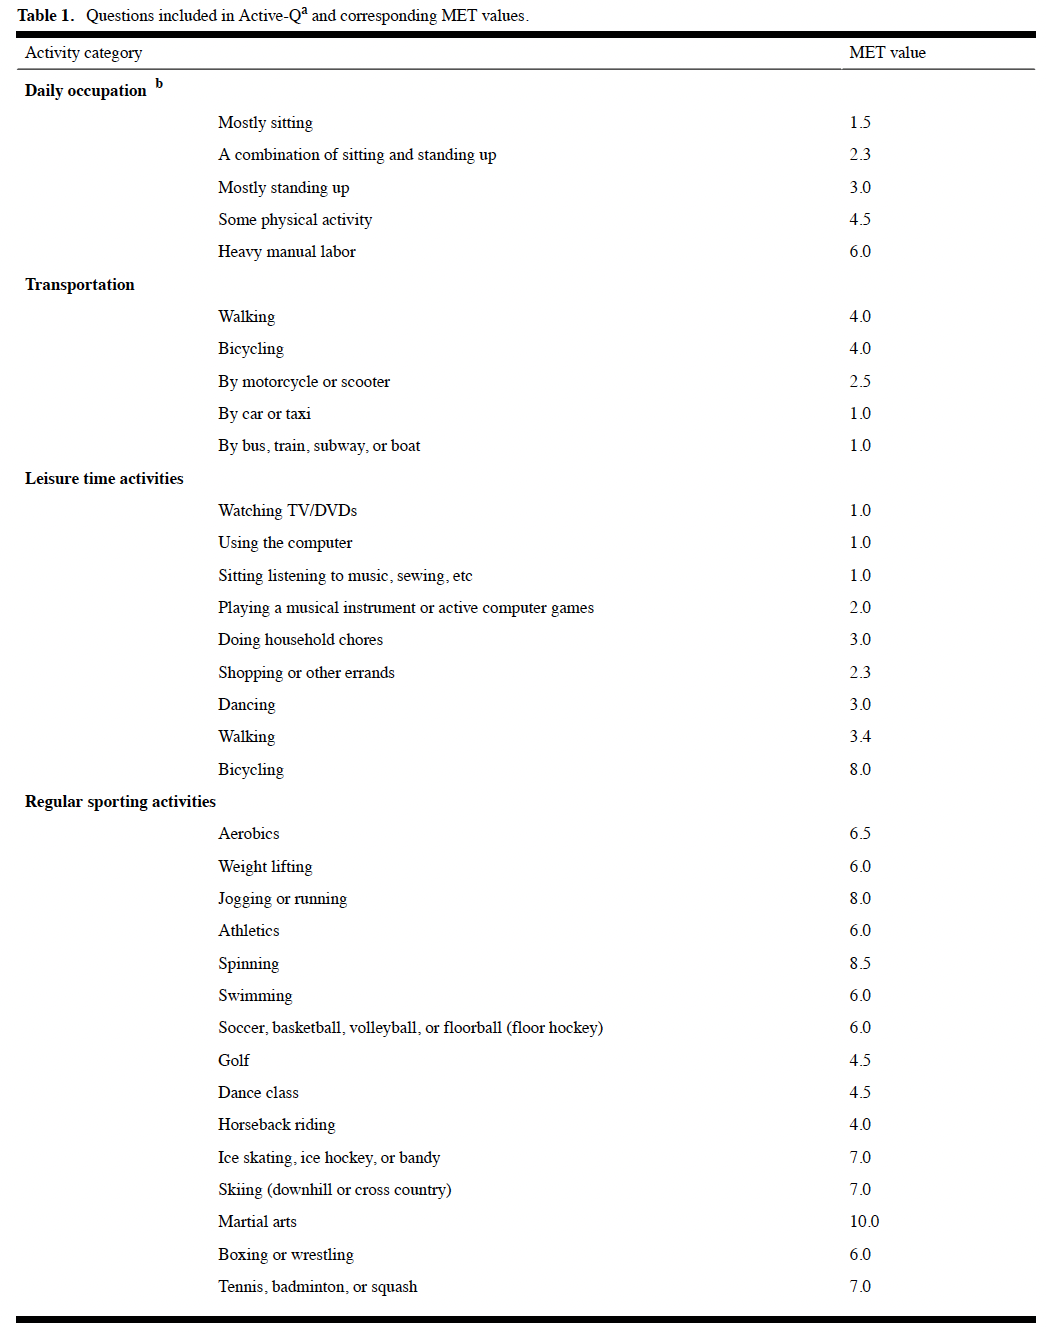
\includegraphics[width=0.8\textwidth]{appendix/met_values.png}
    \caption{MET value labels \parencite{Bonn_2012}}
    \label{fig: met_values}
\end{figure}
\begin{figure}[ht]
    \centering
    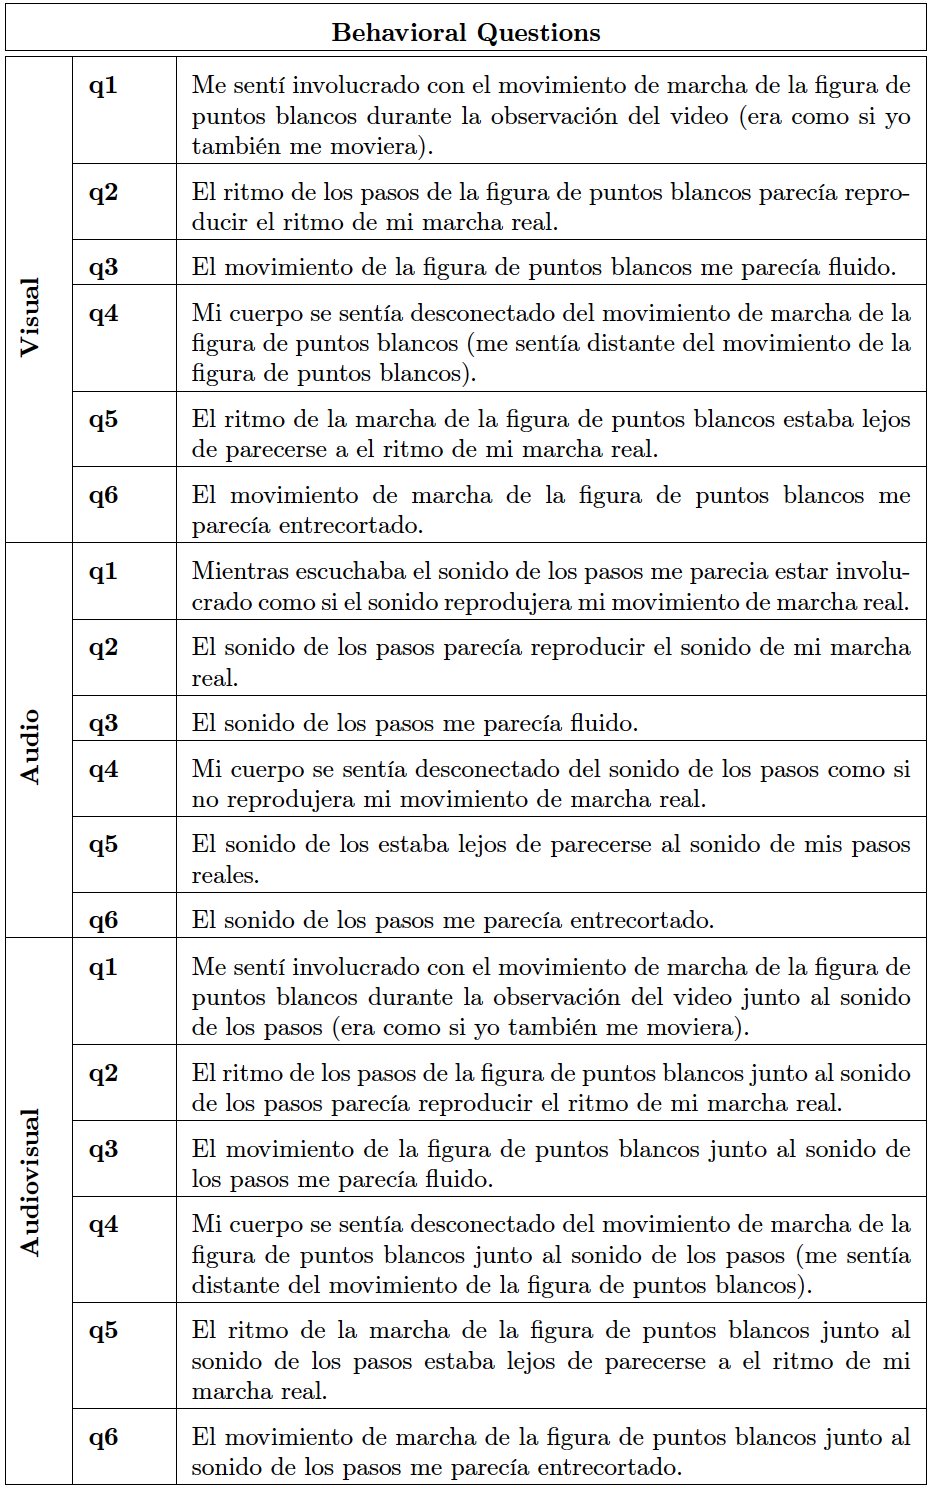
\includegraphics[width=0.70\textwidth]{appendix/questions.png}
    \caption{Behavioral questions translated in English from Spanish}
    \label{fig: Behavioral questions}
\end{figure}

\clearpage
\chapter*{Results}
\section*{Results EEG data}
\subsection*{Signal-To-Noise (SNR)}
\subsubsection*{Control group}
\begin{figure}[H]
    \centering
    \begin{subfigure}[b]{0.48\textwidth}
        \centering
        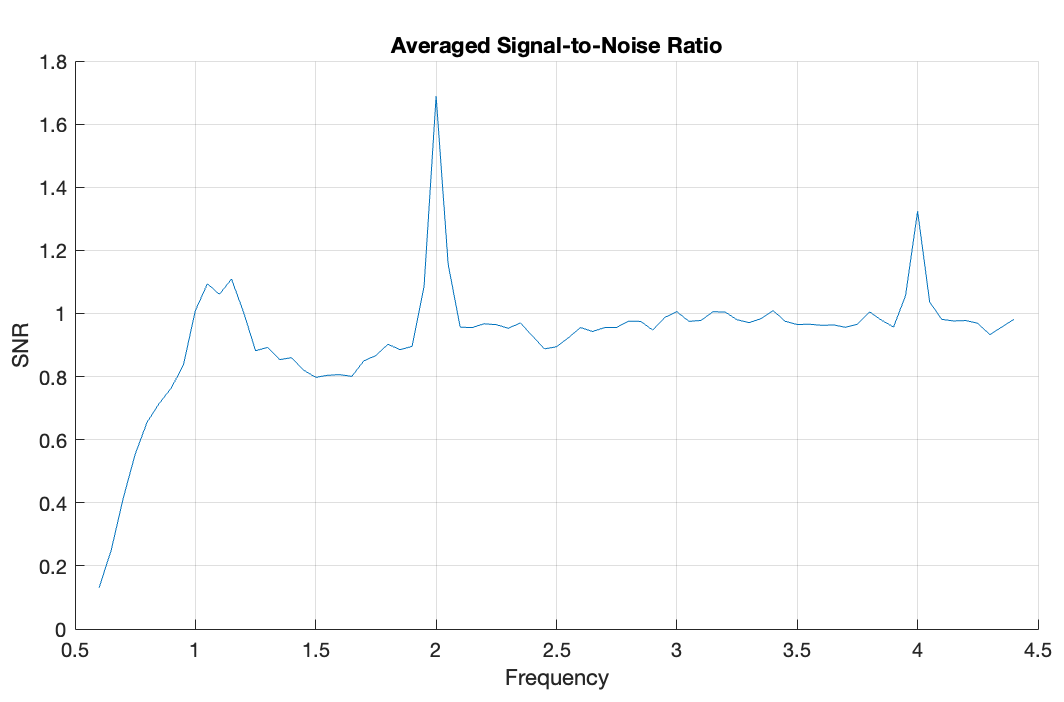
\includegraphics[width=\textwidth]{healthy_images/rhythmic_condition_snr.png}
        \caption{SNR in the rhythmic condition}
        \label{fig: snr_rhythmic: control}
    \end{subfigure}
    \hfill
    \begin{subfigure}[b]{0.48\textwidth}
        \centering
        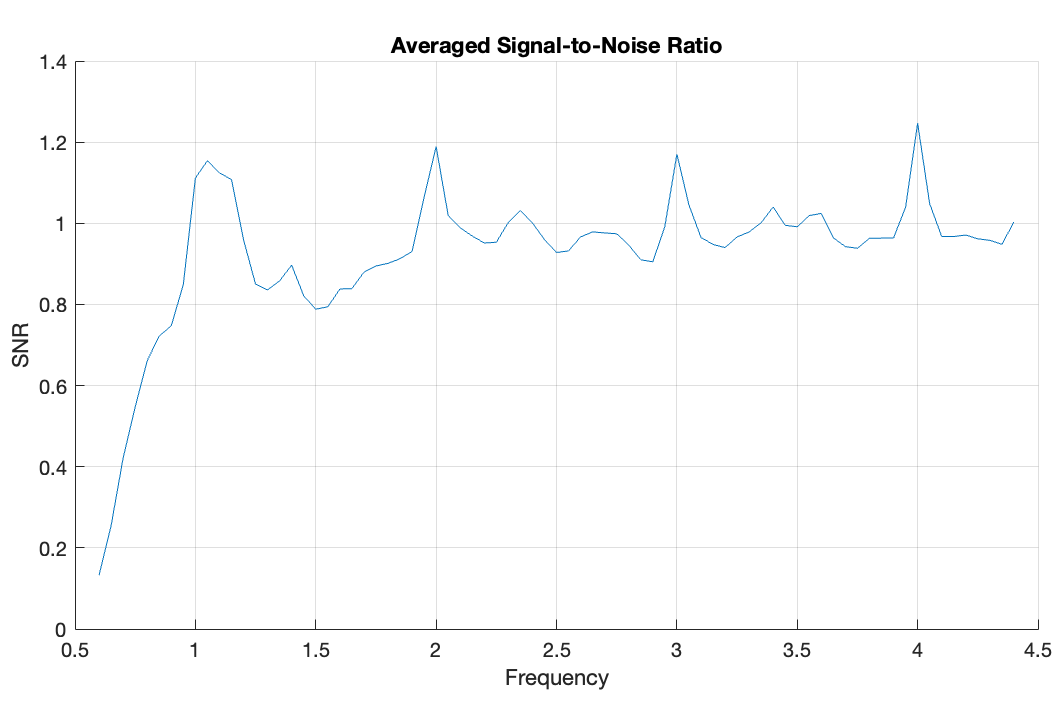
\includegraphics[width=\textwidth]{healthy_images/random_condition_snr.png}
        \caption{SNR in the random condition}
        \label{fig: snr_random: control}
    \end{subfigure}
    \caption{SNR comparison in the control group}
    \label{fig: snr_control_group}
\end{figure}

\subsubsection*{Stroke group}
\begin{figure}[H]
    \centering
    \begin{subfigure}[b]{0.48\textwidth}
        \centering
        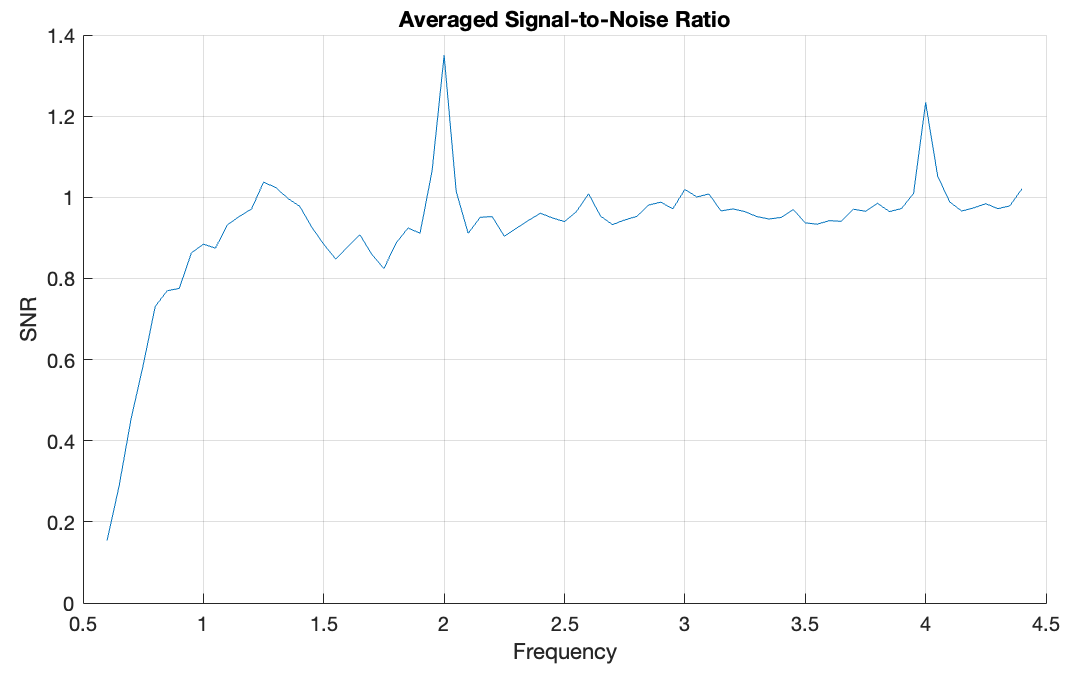
\includegraphics[width=\textwidth]{stroke_images/rhythmic_snr.png}
        \caption{SNR in the rhythmic condition}
        \label{fig: snr_rhythmic: stroke}
    \end{subfigure}
    \hfill
    \begin{subfigure}[b]{0.48\textwidth}
        \centering
        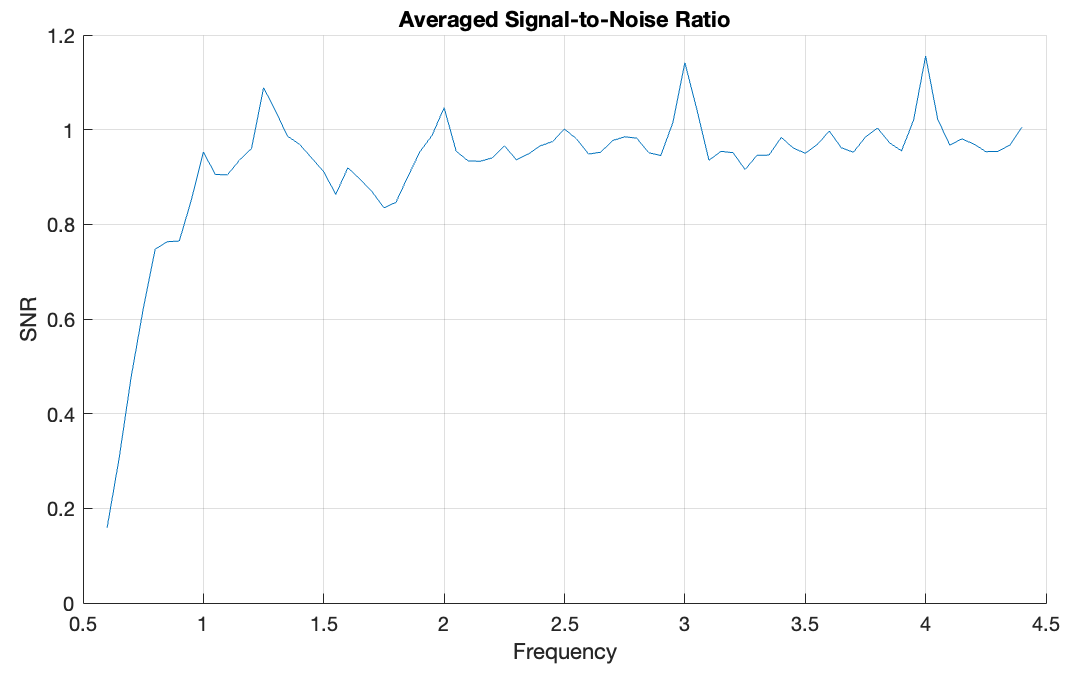
\includegraphics[width=\textwidth]{stroke_images/random_snr.png}
        \caption{SNR in the random condition}
        \label{fig: snr_random: stroke}
    \end{subfigure}
    \caption{SNR comparison in the stroke group}
    \label{fig: snr_stroke_group}
\end{figure}

\clearpage
\subsection*{Activity power spectrum}
\subsubsection*{Control group}
\begin{figure}[H]
    \centering
    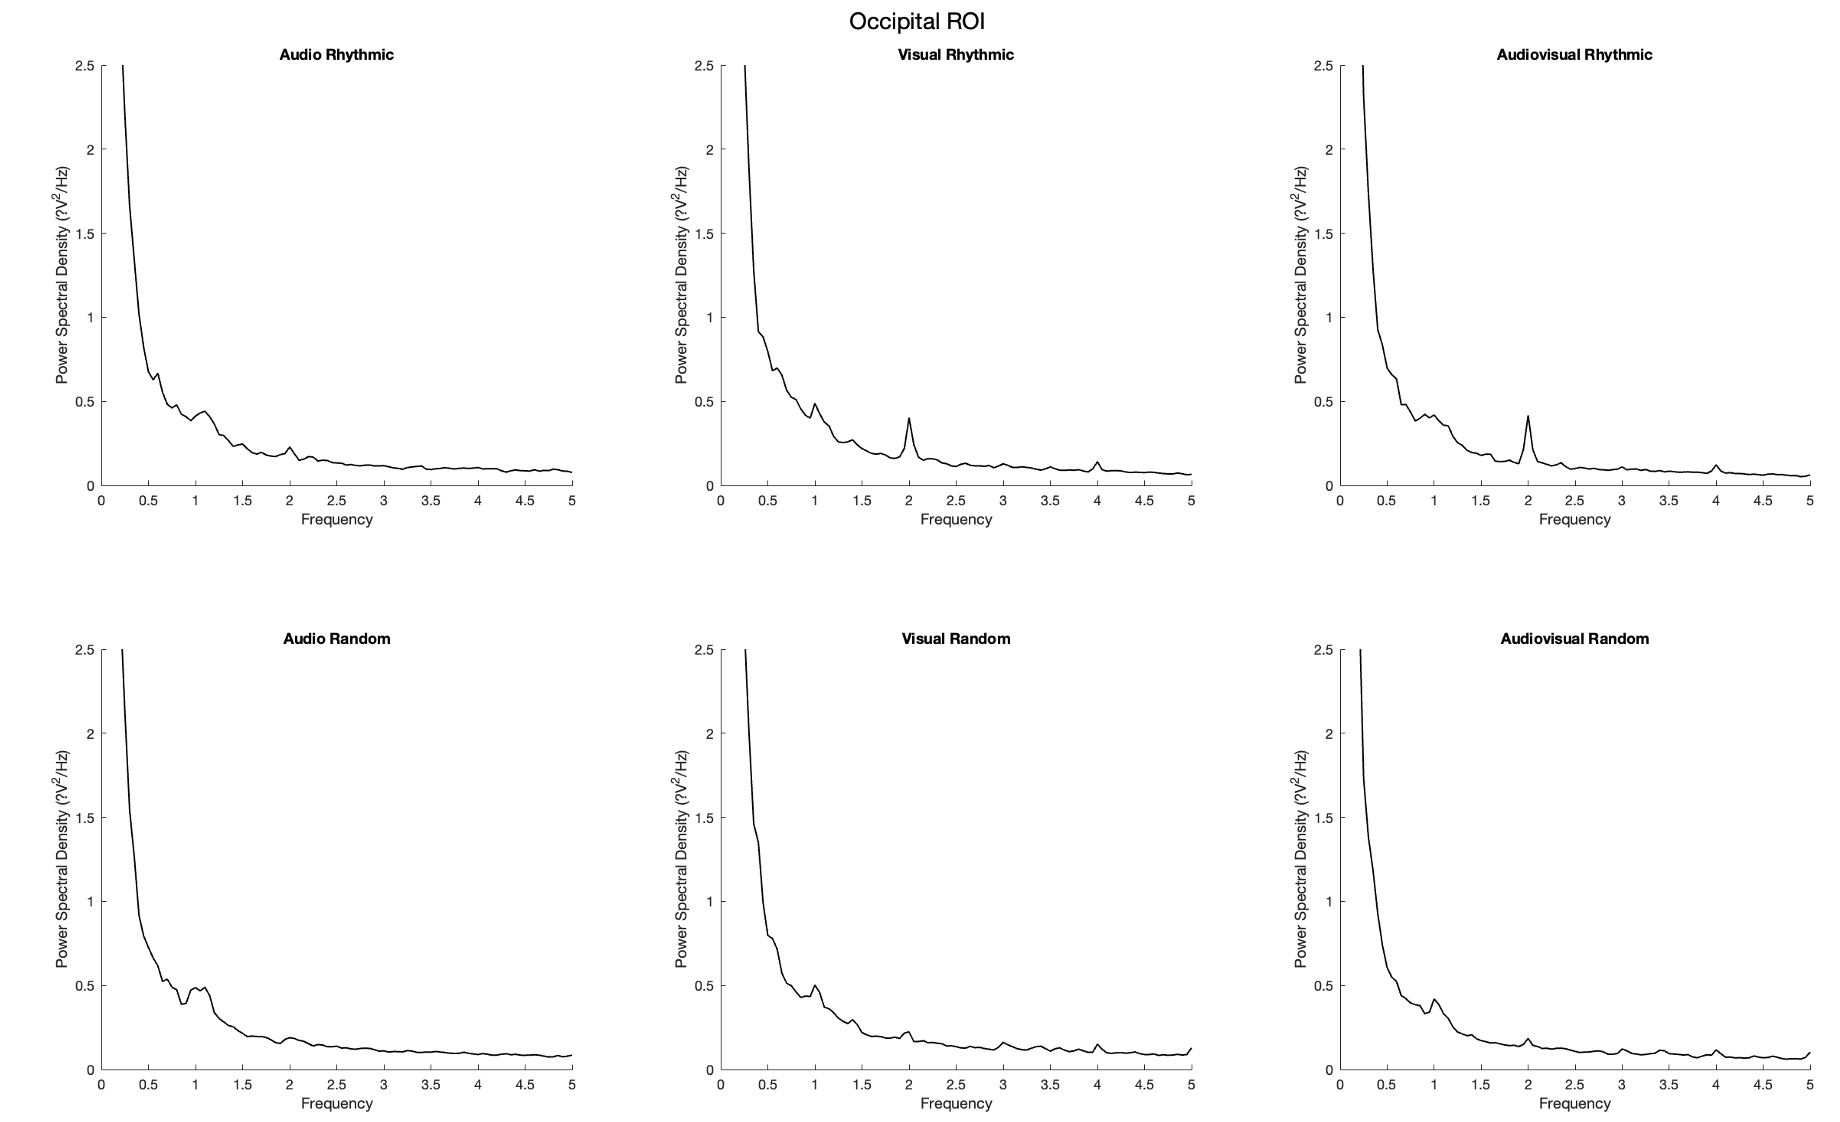
\includegraphics[width=0.85\textwidth]{healthy_images/occipitalROI_graph.png}
    \caption{Activity power spectrum in the occipital ROI}
    \label{fig: occipital ROI: control}
\end{figure}
\begin{figure}[H]
    \centering
    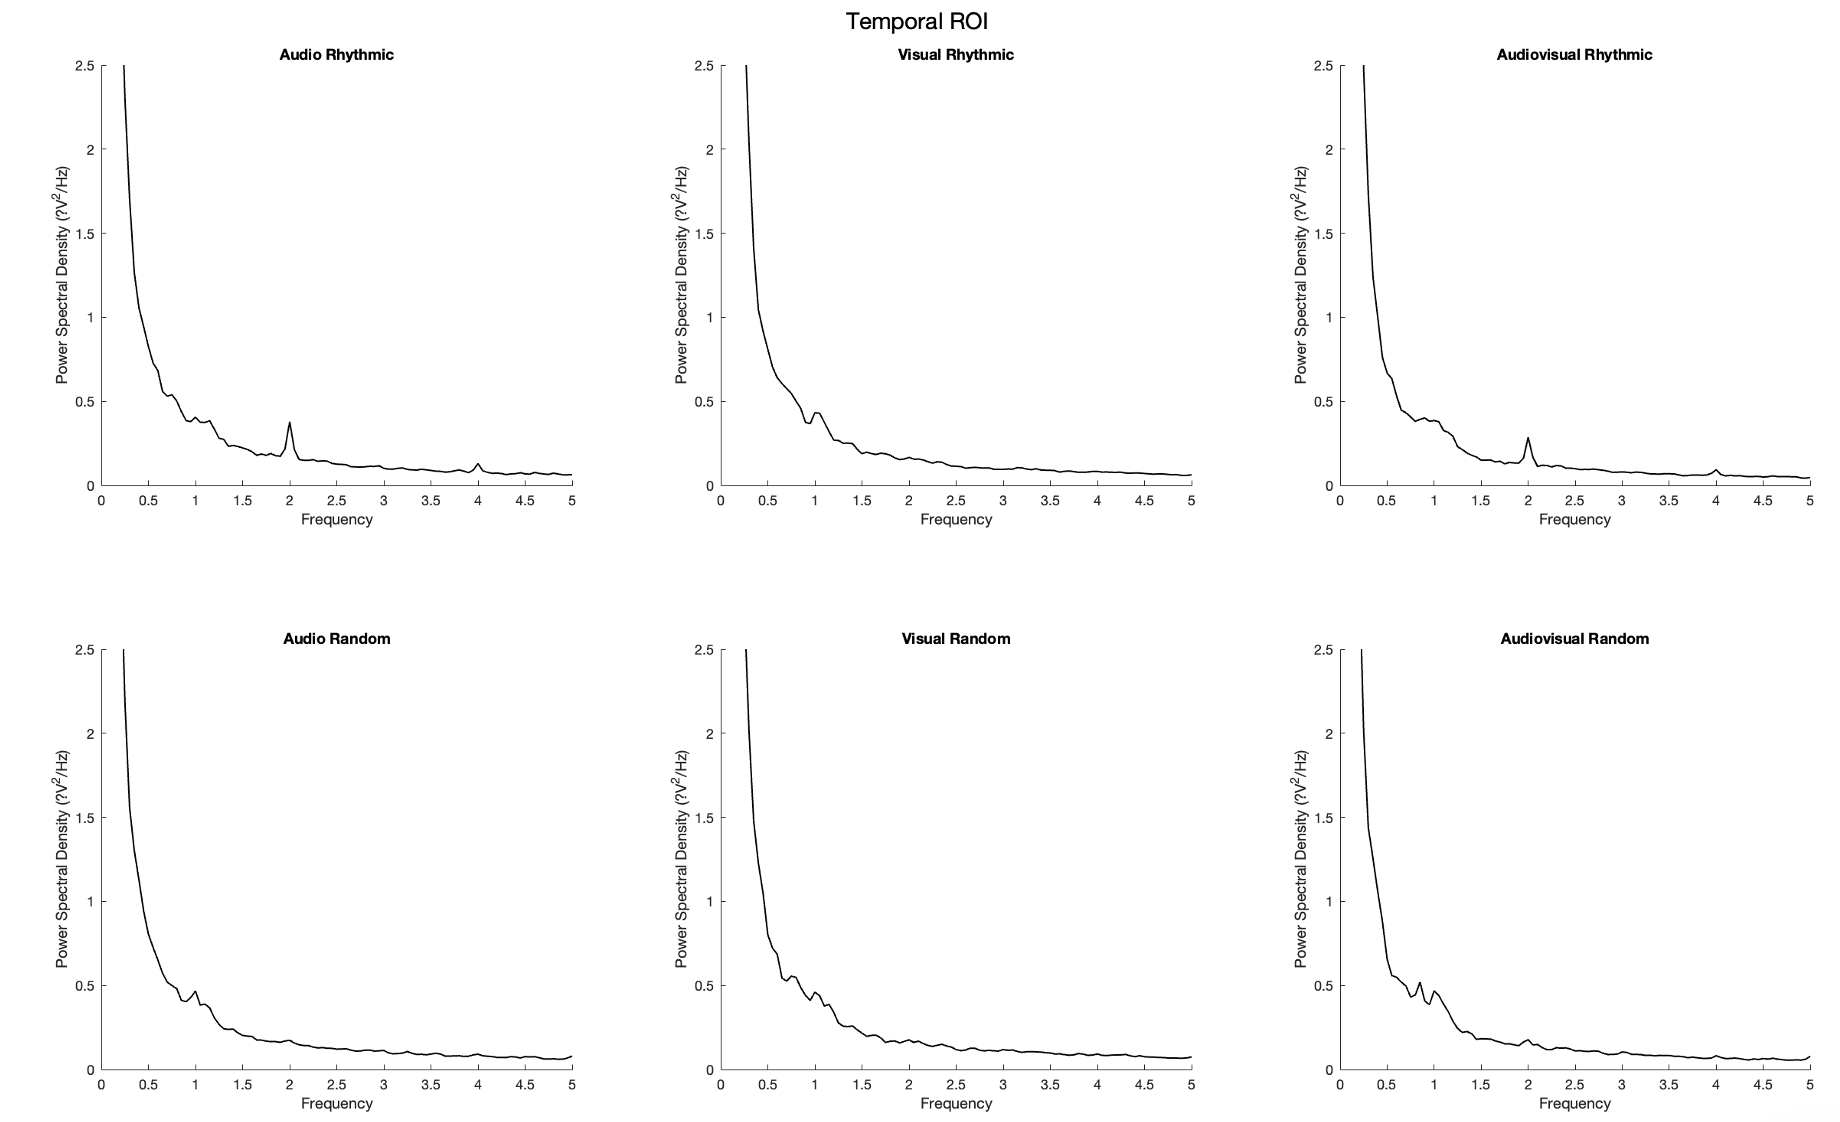
\includegraphics[width=0.85\textwidth]{healthy_images/temporalROI_graph.png}
    \caption{Activity power spectrum  in the temporal ROI}
    \label{fig: temporal ROI: control}
\end{figure}
\begin{figure}[H]
    \centering
    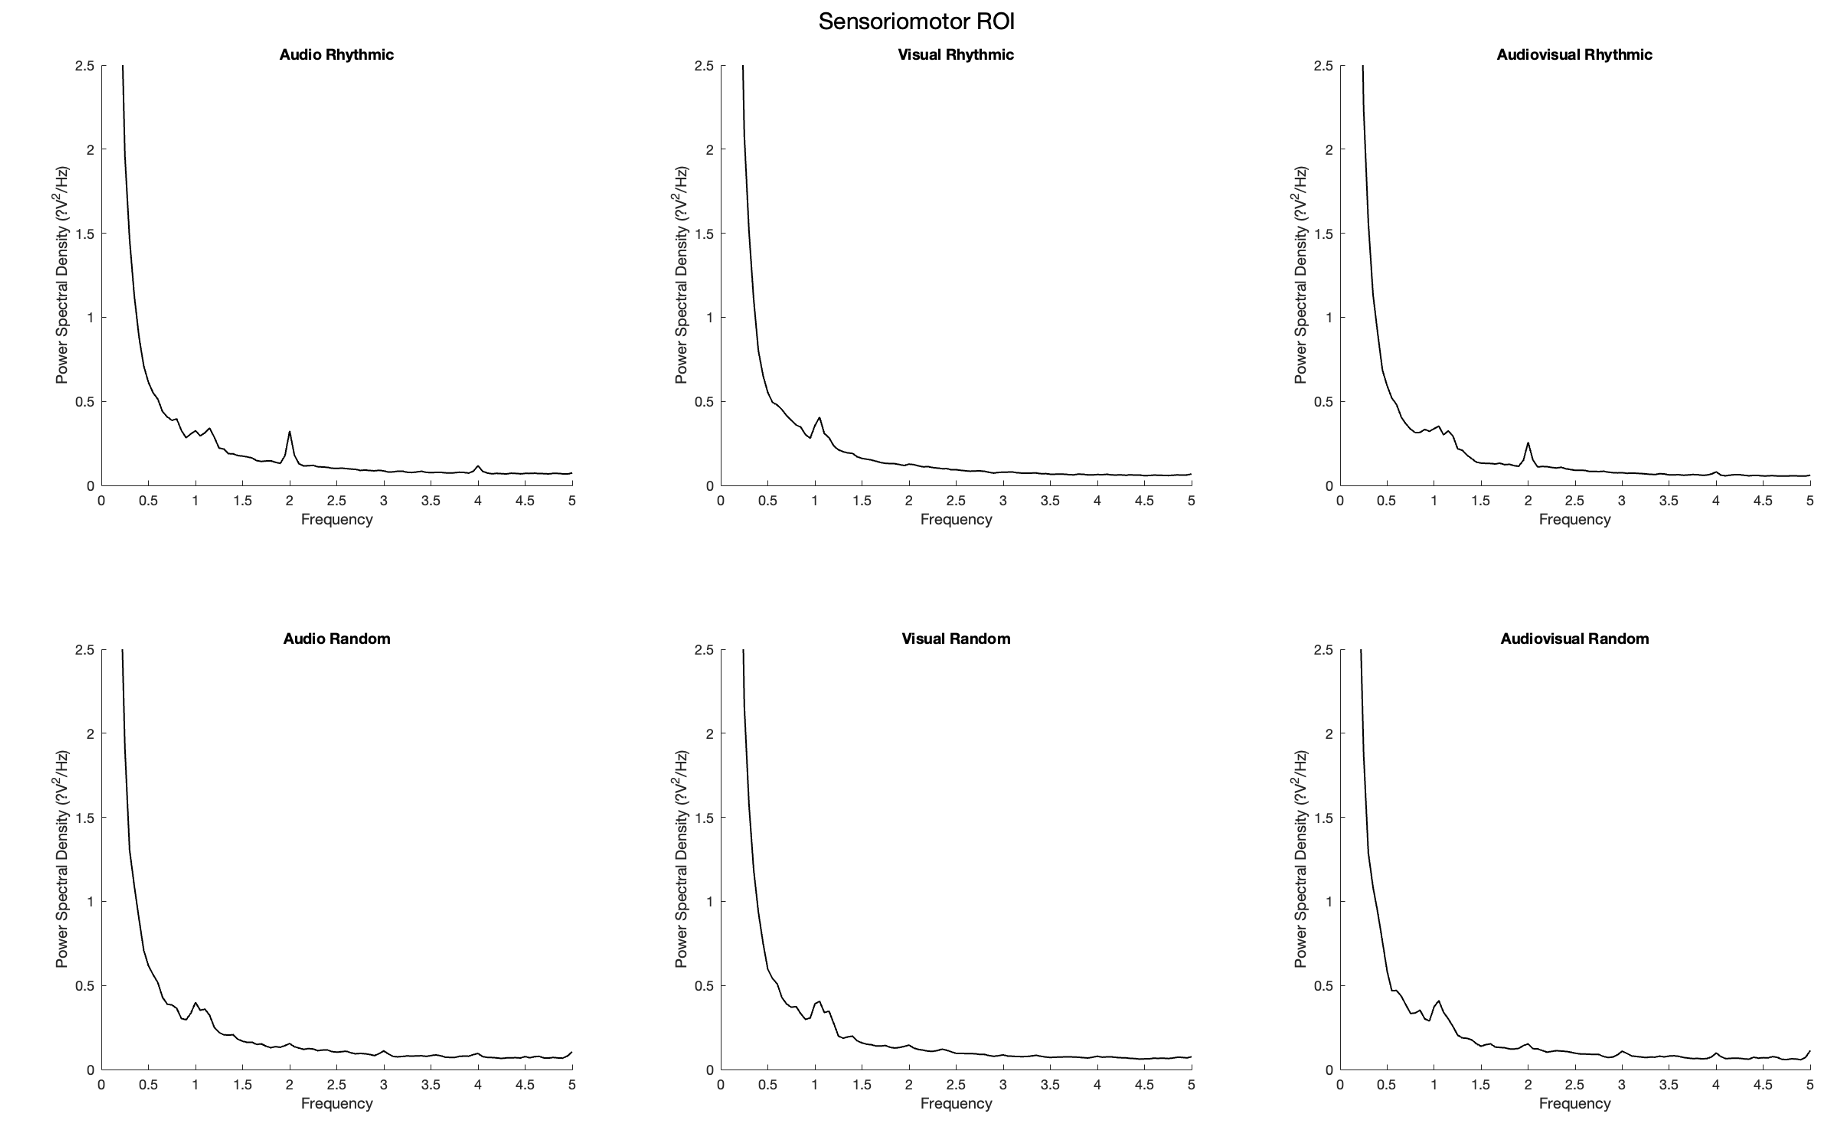
\includegraphics[width=0.85\textwidth]{healthy_images/sensorimotorROI_graph.png}
    \caption{Activity power spectrum in the sensorimotor ROI}
    \label{fig: sensorimotor ROI: control} 
\end{figure} 

\subsubsection*{Stroke group}
\begin{figure}[H]
    \centering
    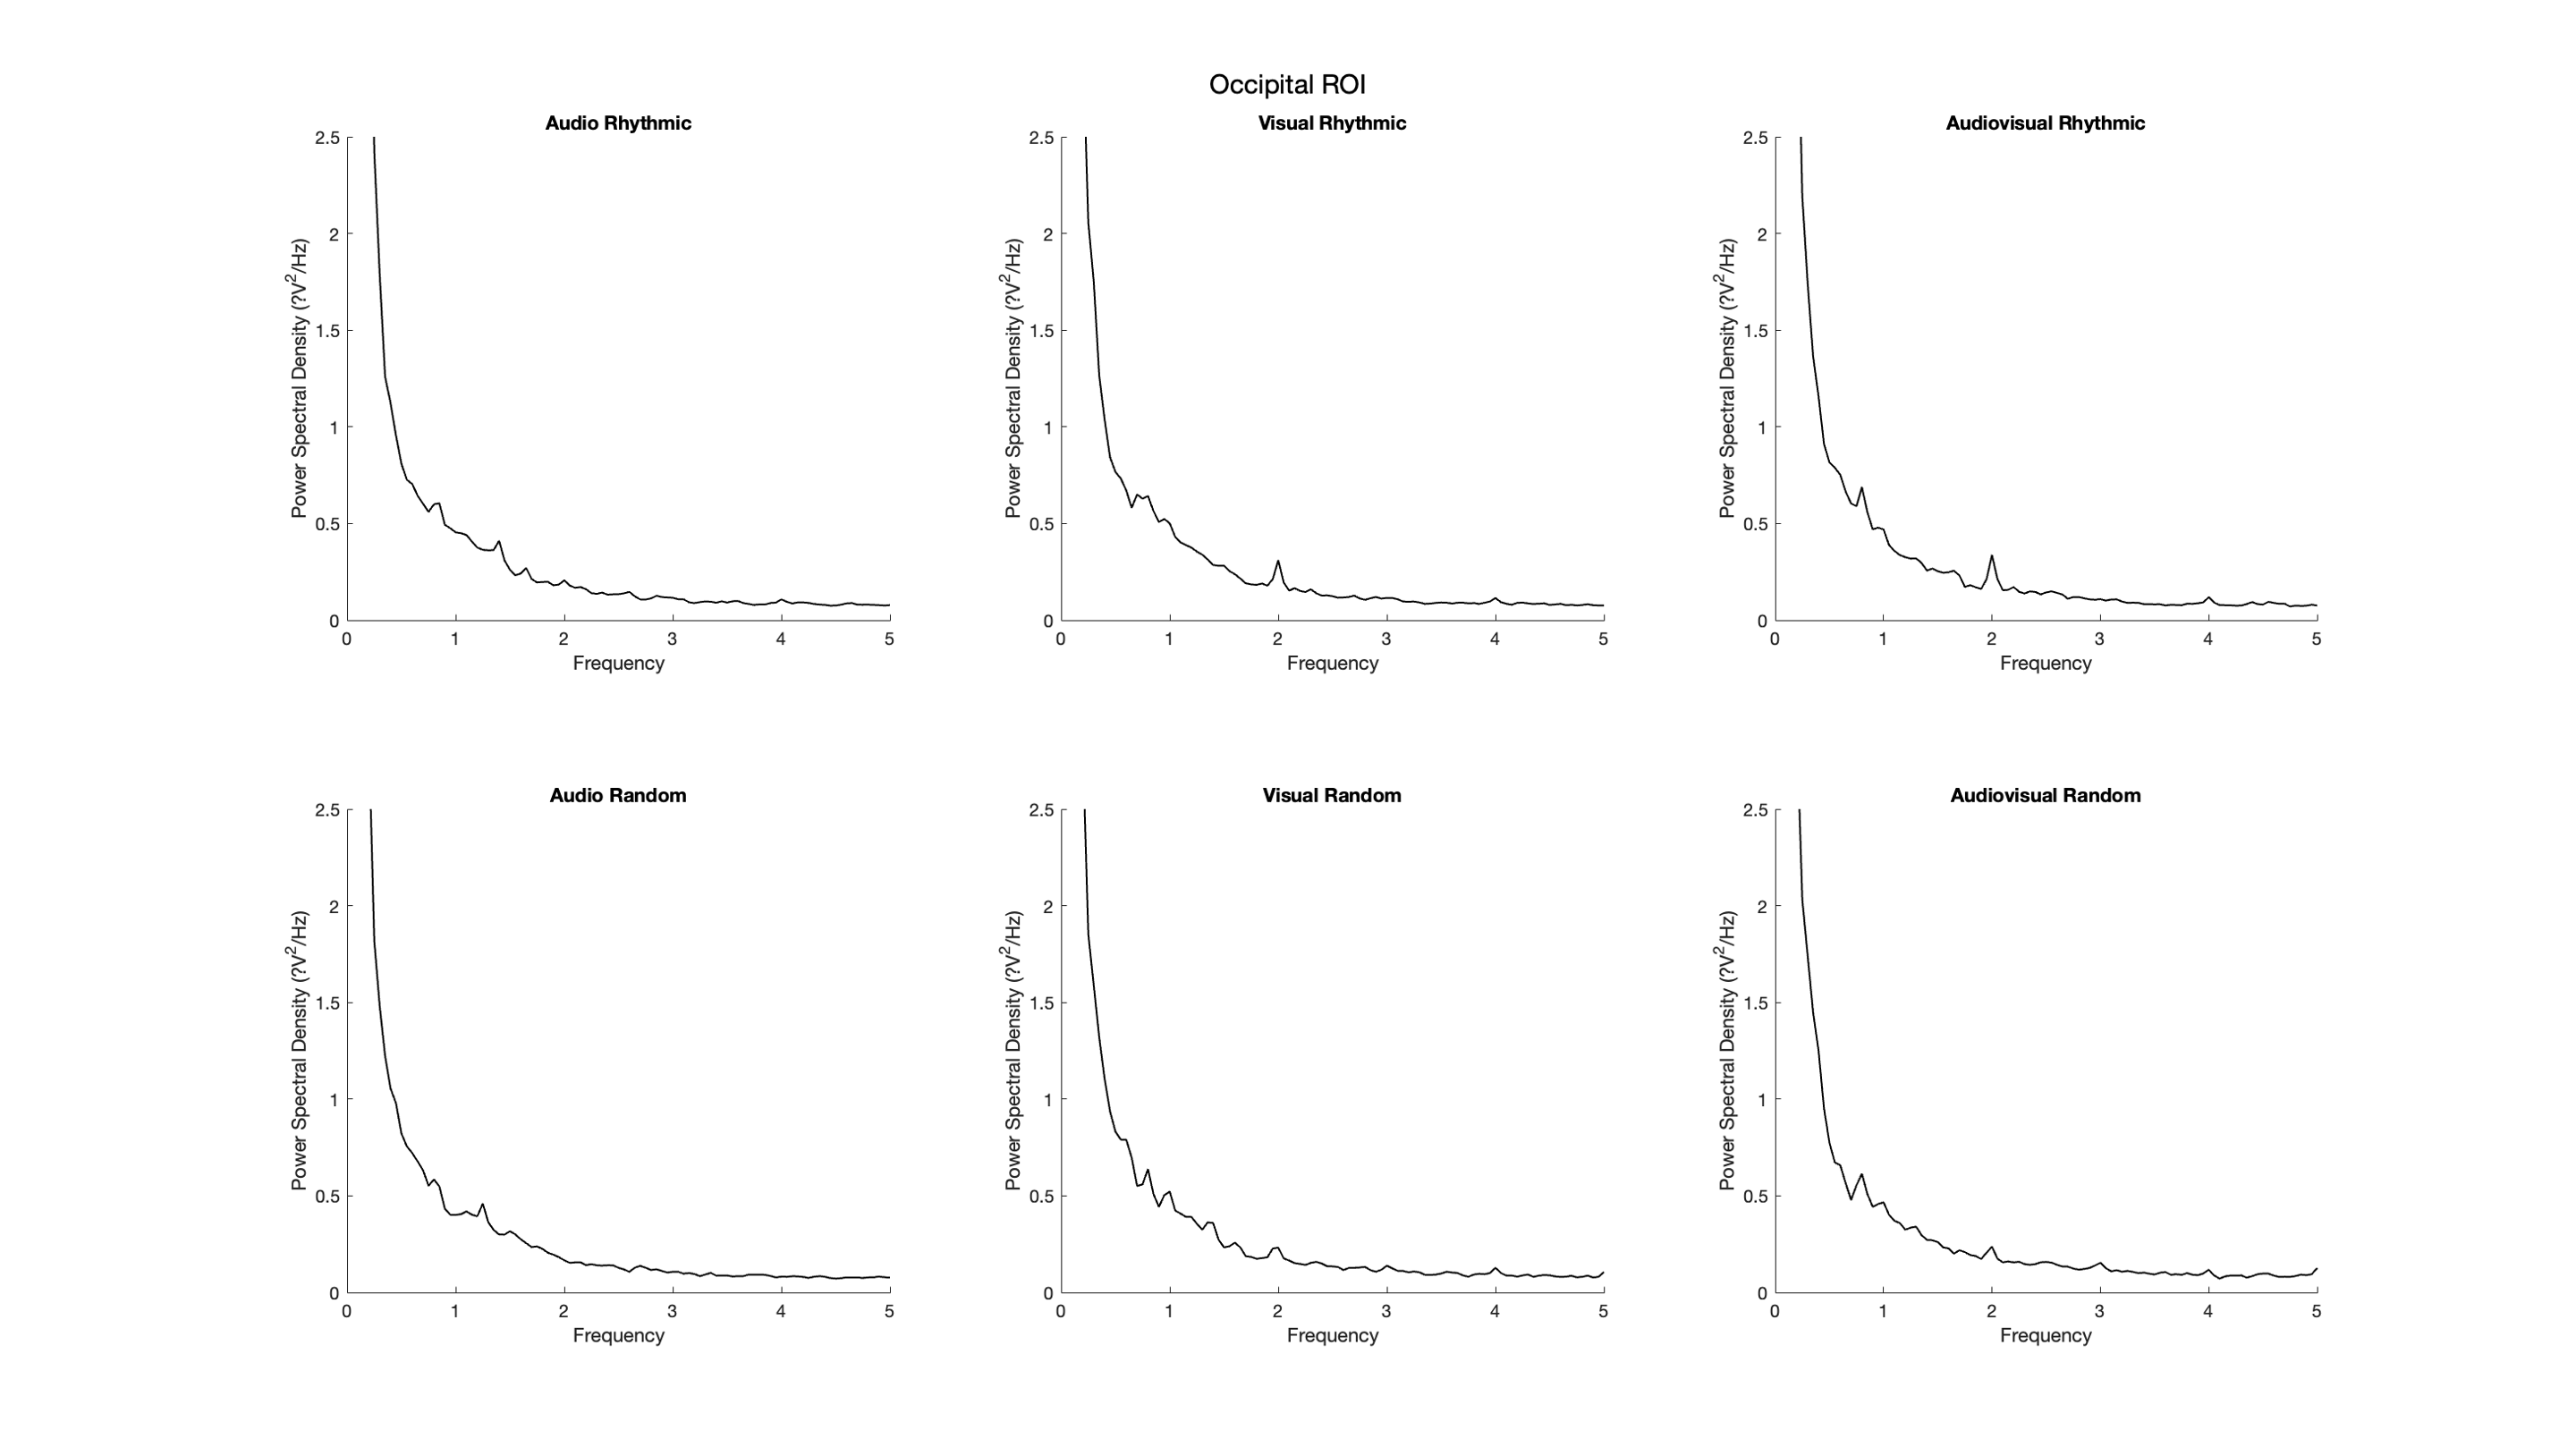
\includegraphics[width=0.95\textwidth]{stroke_images/occipital_roi.png}
    \caption{Activity power spectrum in the occipital ROI: stroke group}
    \label{fig: occipital ROI: stroke}
\end{figure}
\begin{figure}[H]
    \centering
    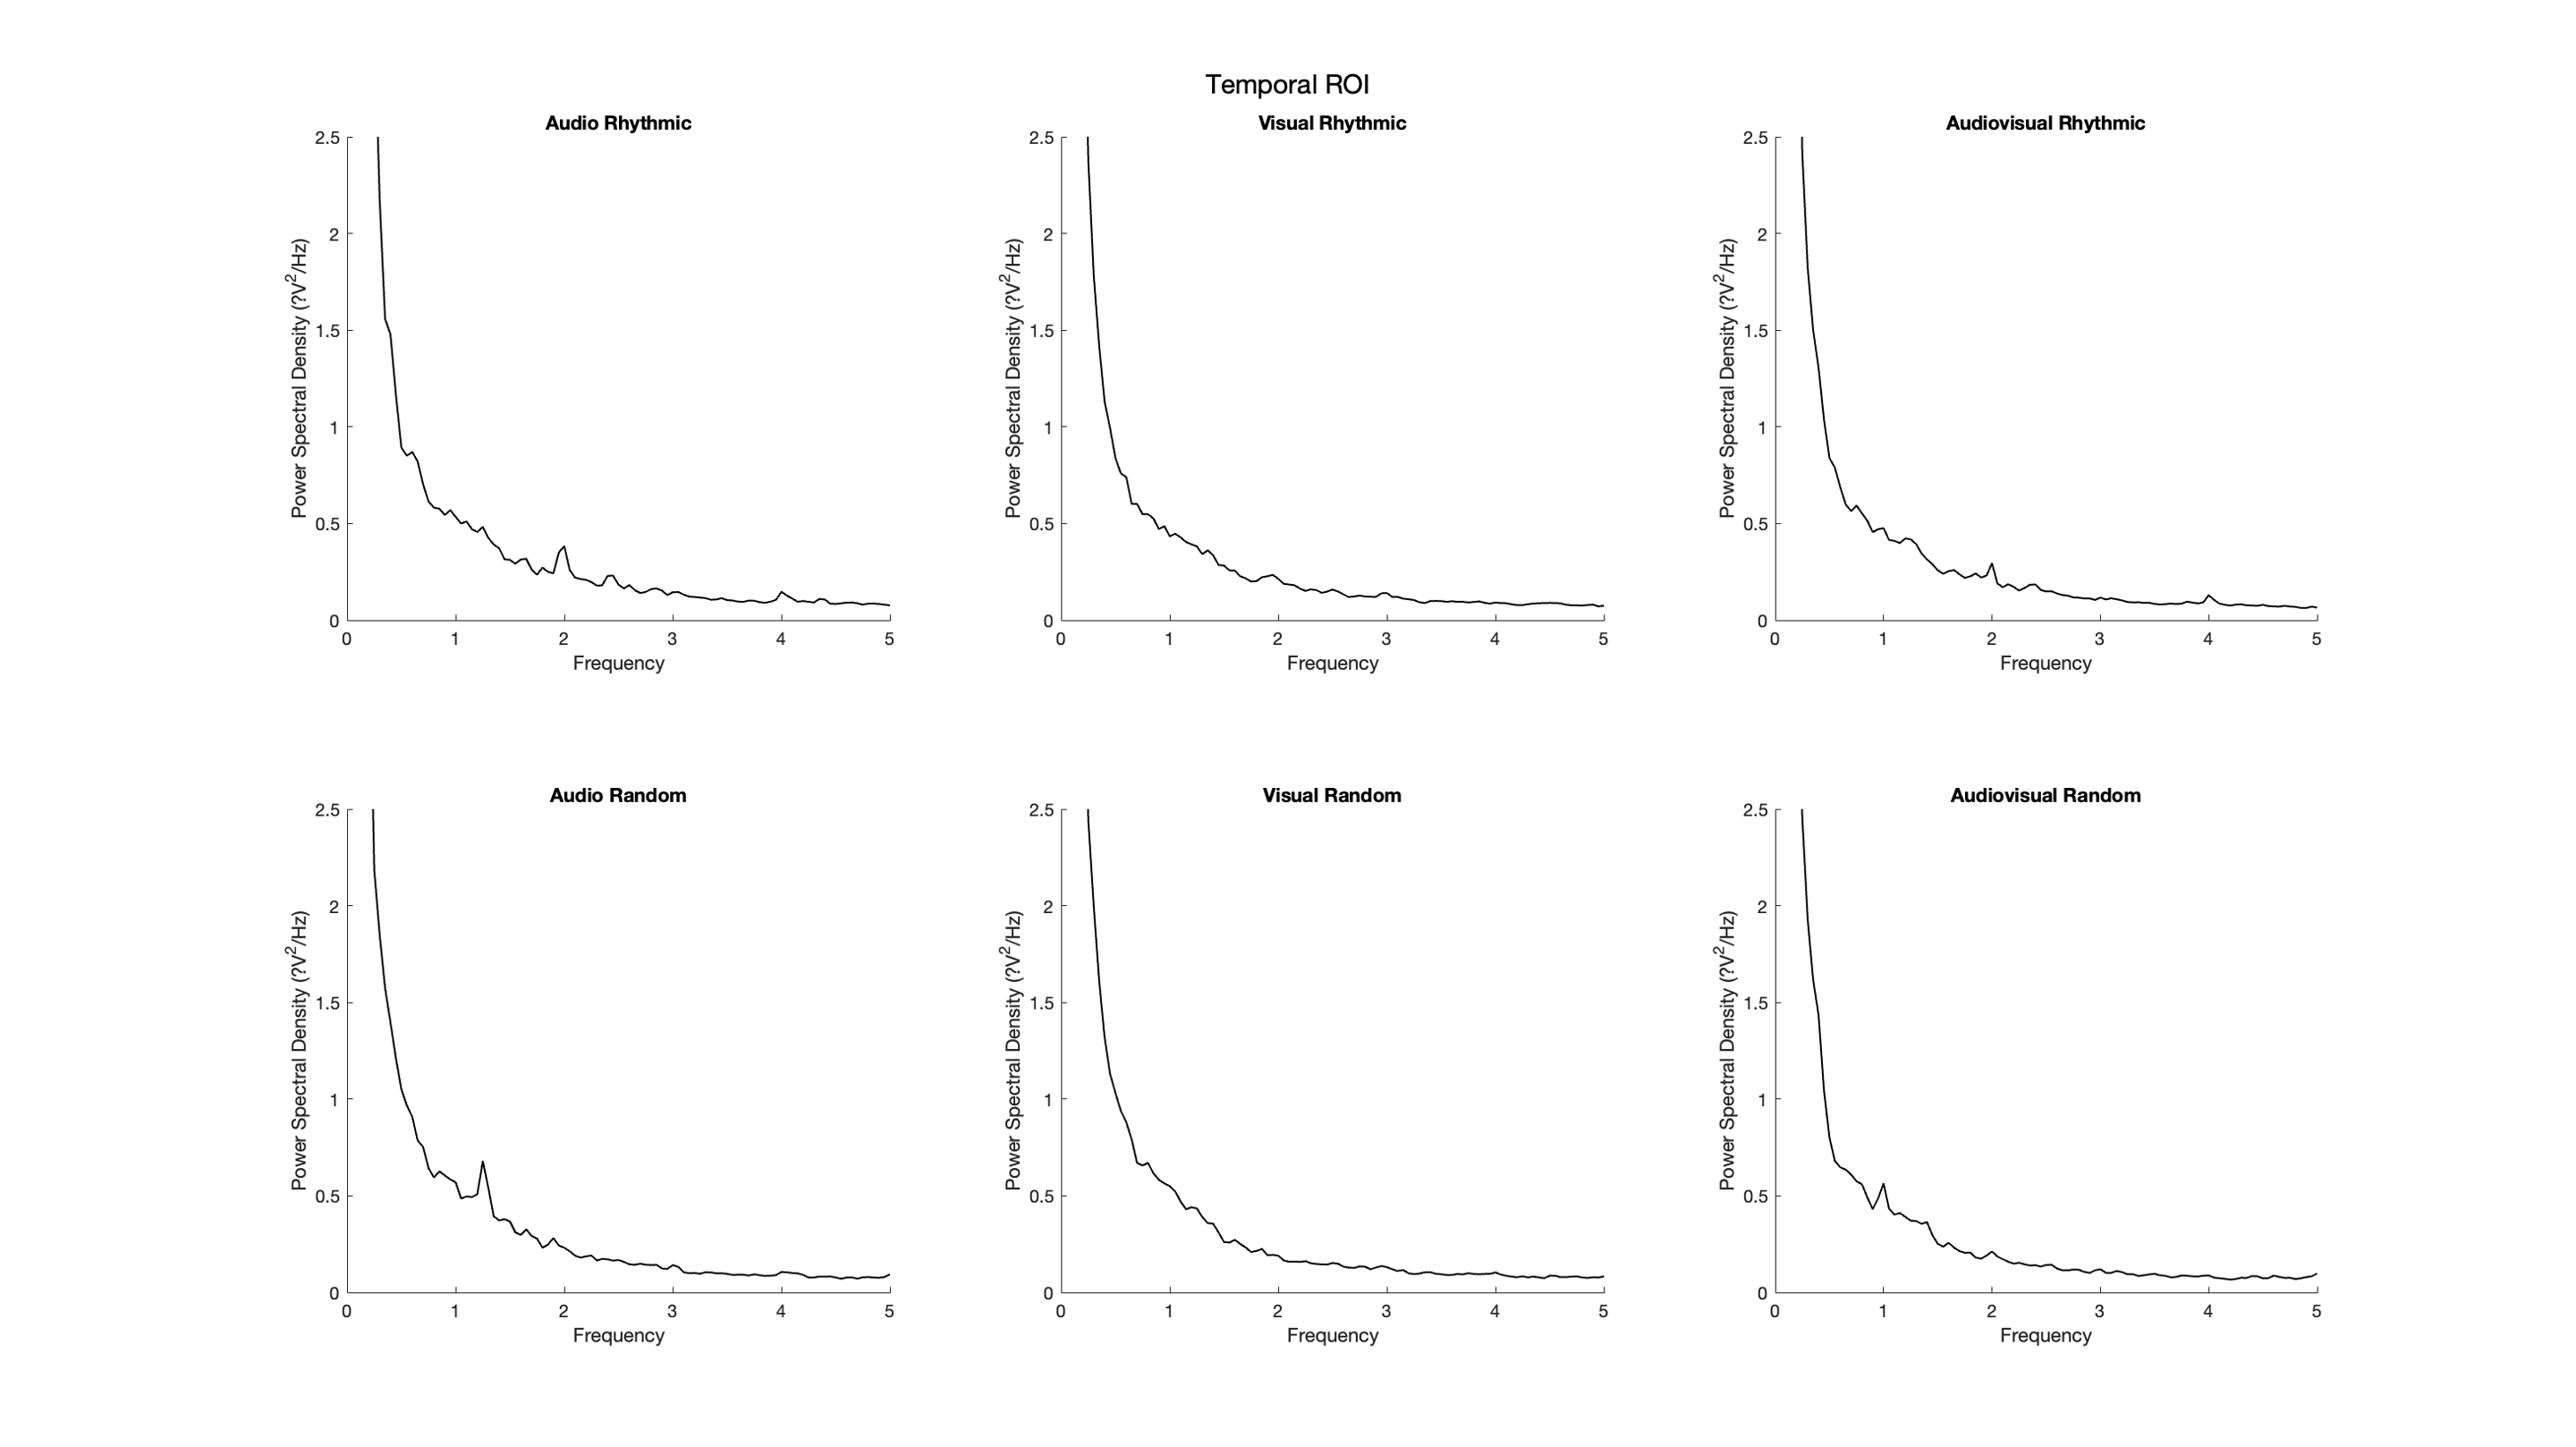
\includegraphics[width=0.95\textwidth]{stroke_images/temporal_roi.png}
    \caption{Activity power spectrum in the temporal ROI:stroke group}
    \label{fig: temporal ROI: stroke}
\end{figure}
\begin{figure}[H]
    \centering
    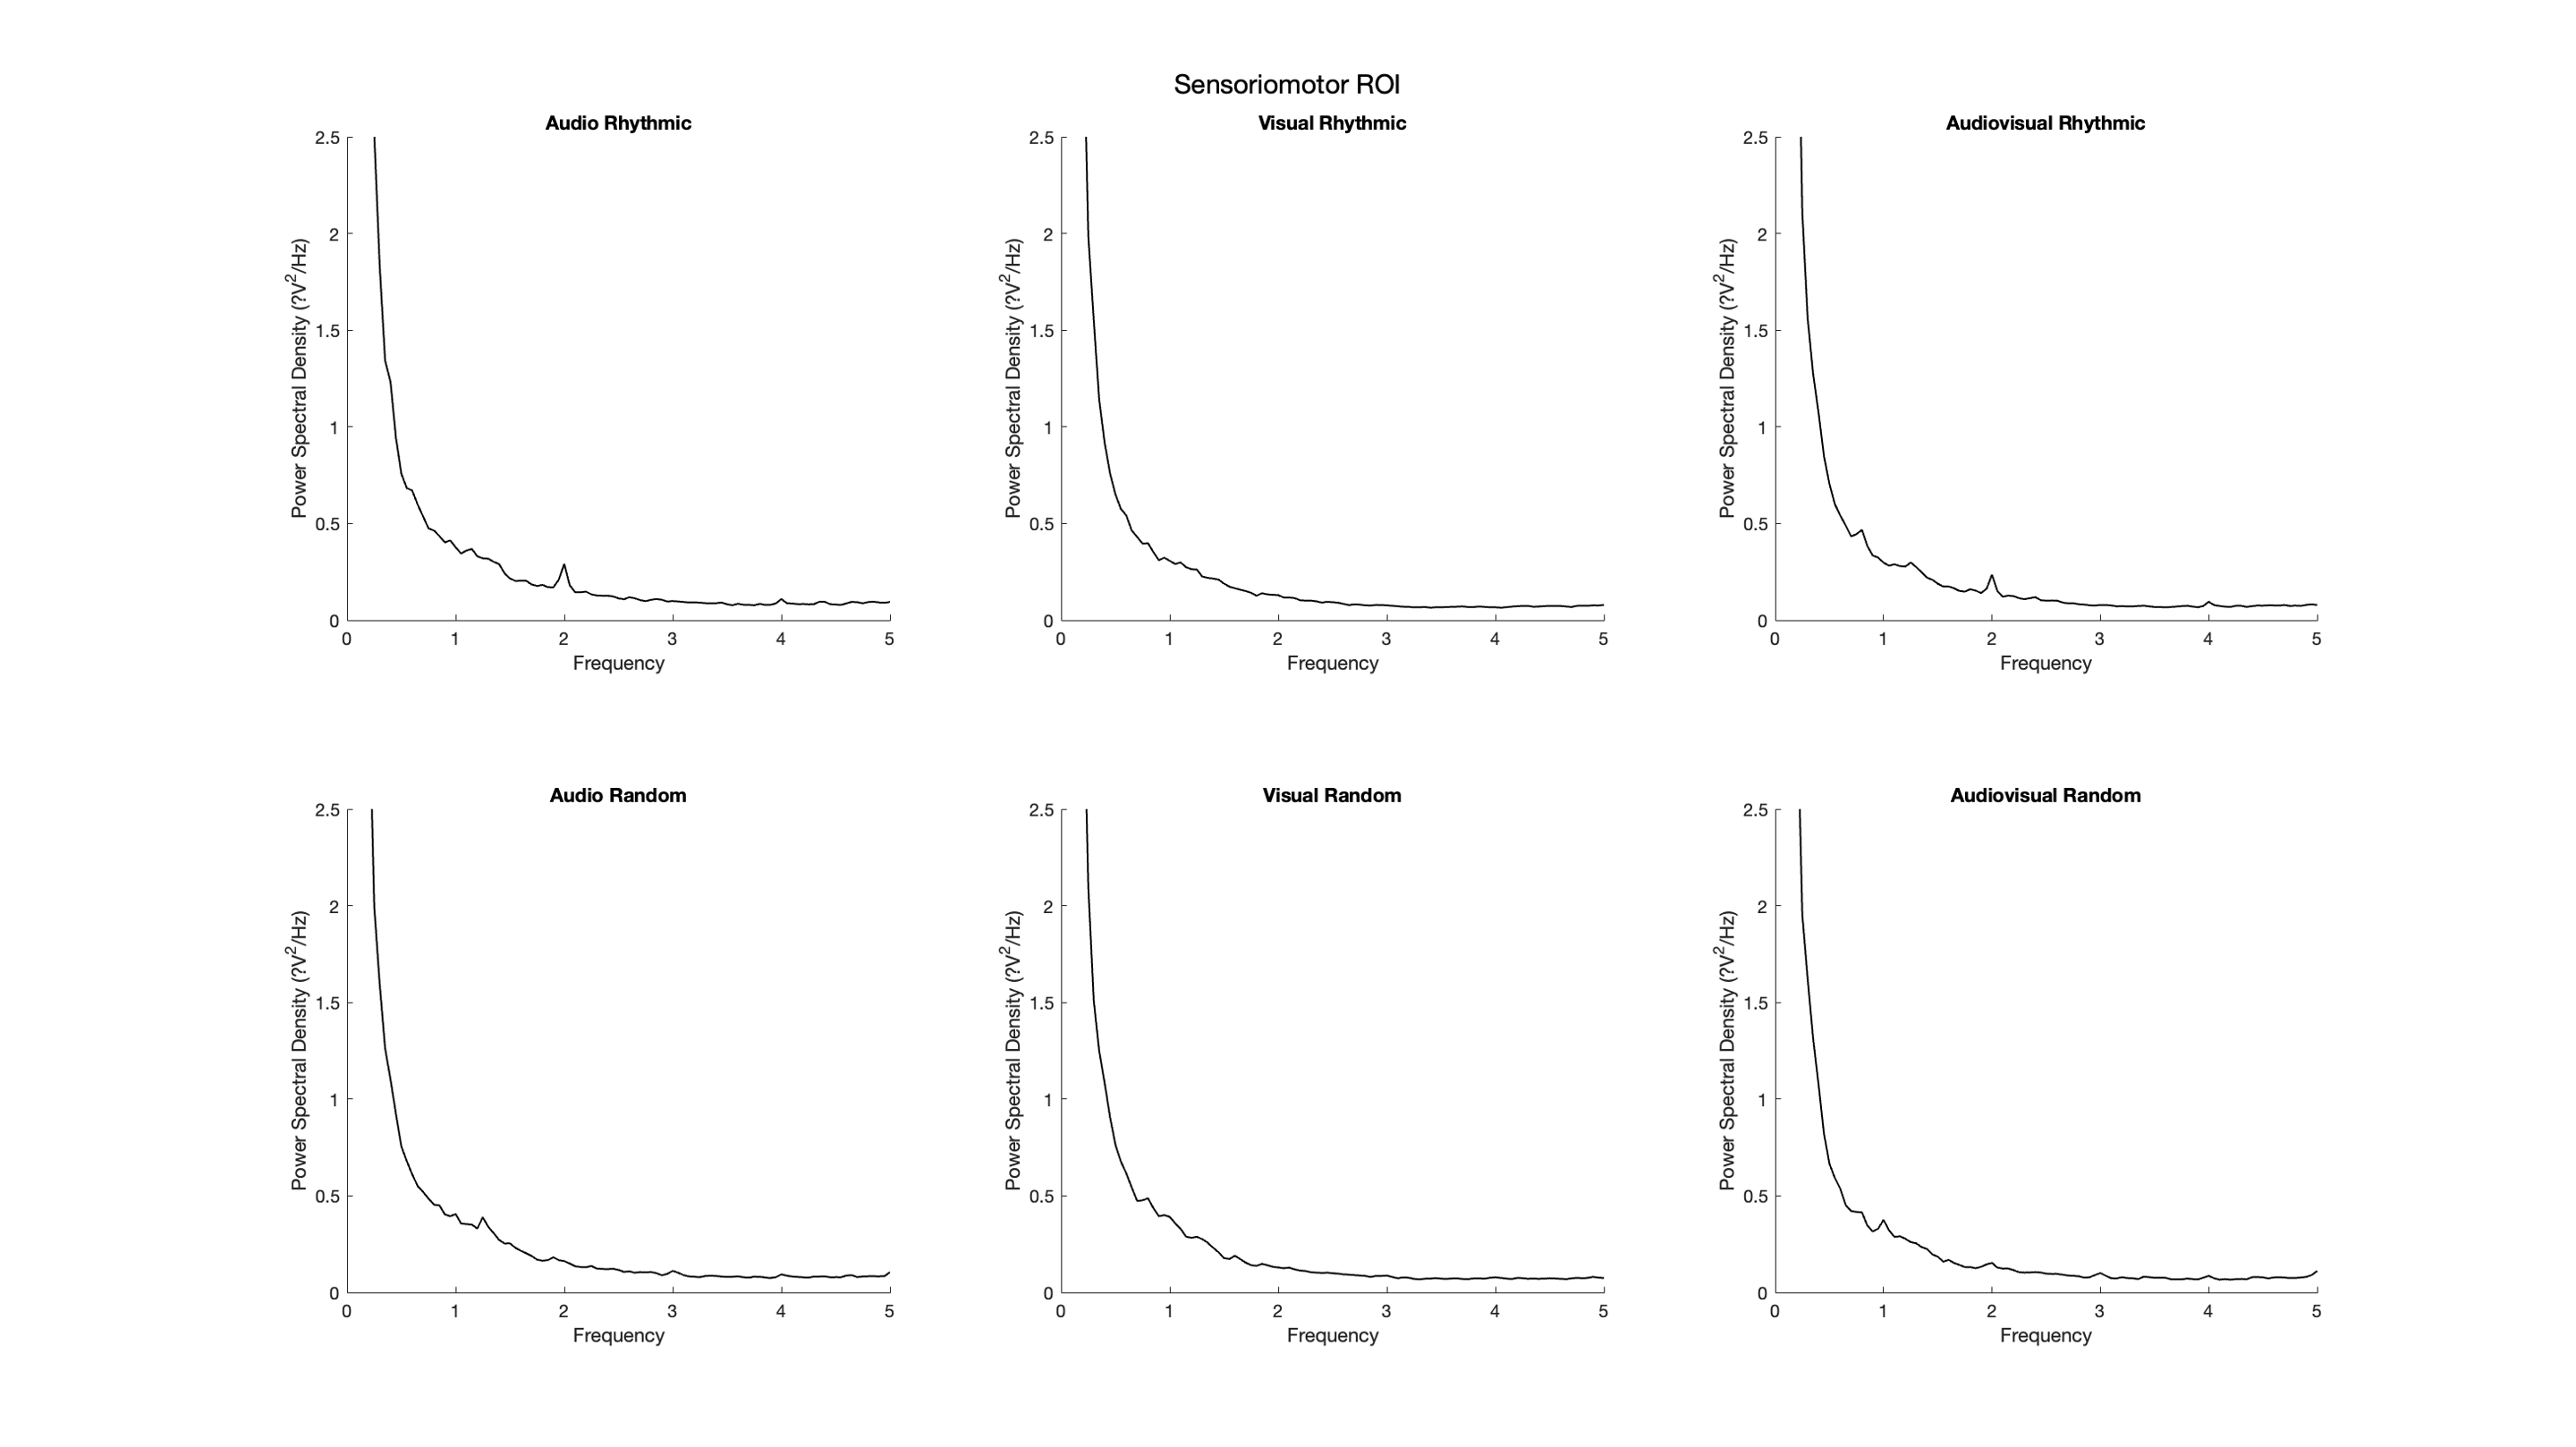
\includegraphics[width=0.95\textwidth]{stroke_images/sensorimotor_roi.png}
    \caption{Activity power spectrum in the sensorimotor ROI: stroke group}
    \label{fig: sensorimotor ROI: stroke} 
\end{figure} 
\vfill

\clearpage
\subsection*{Topographies}
\begin{figure}[htbp]
    \centering
    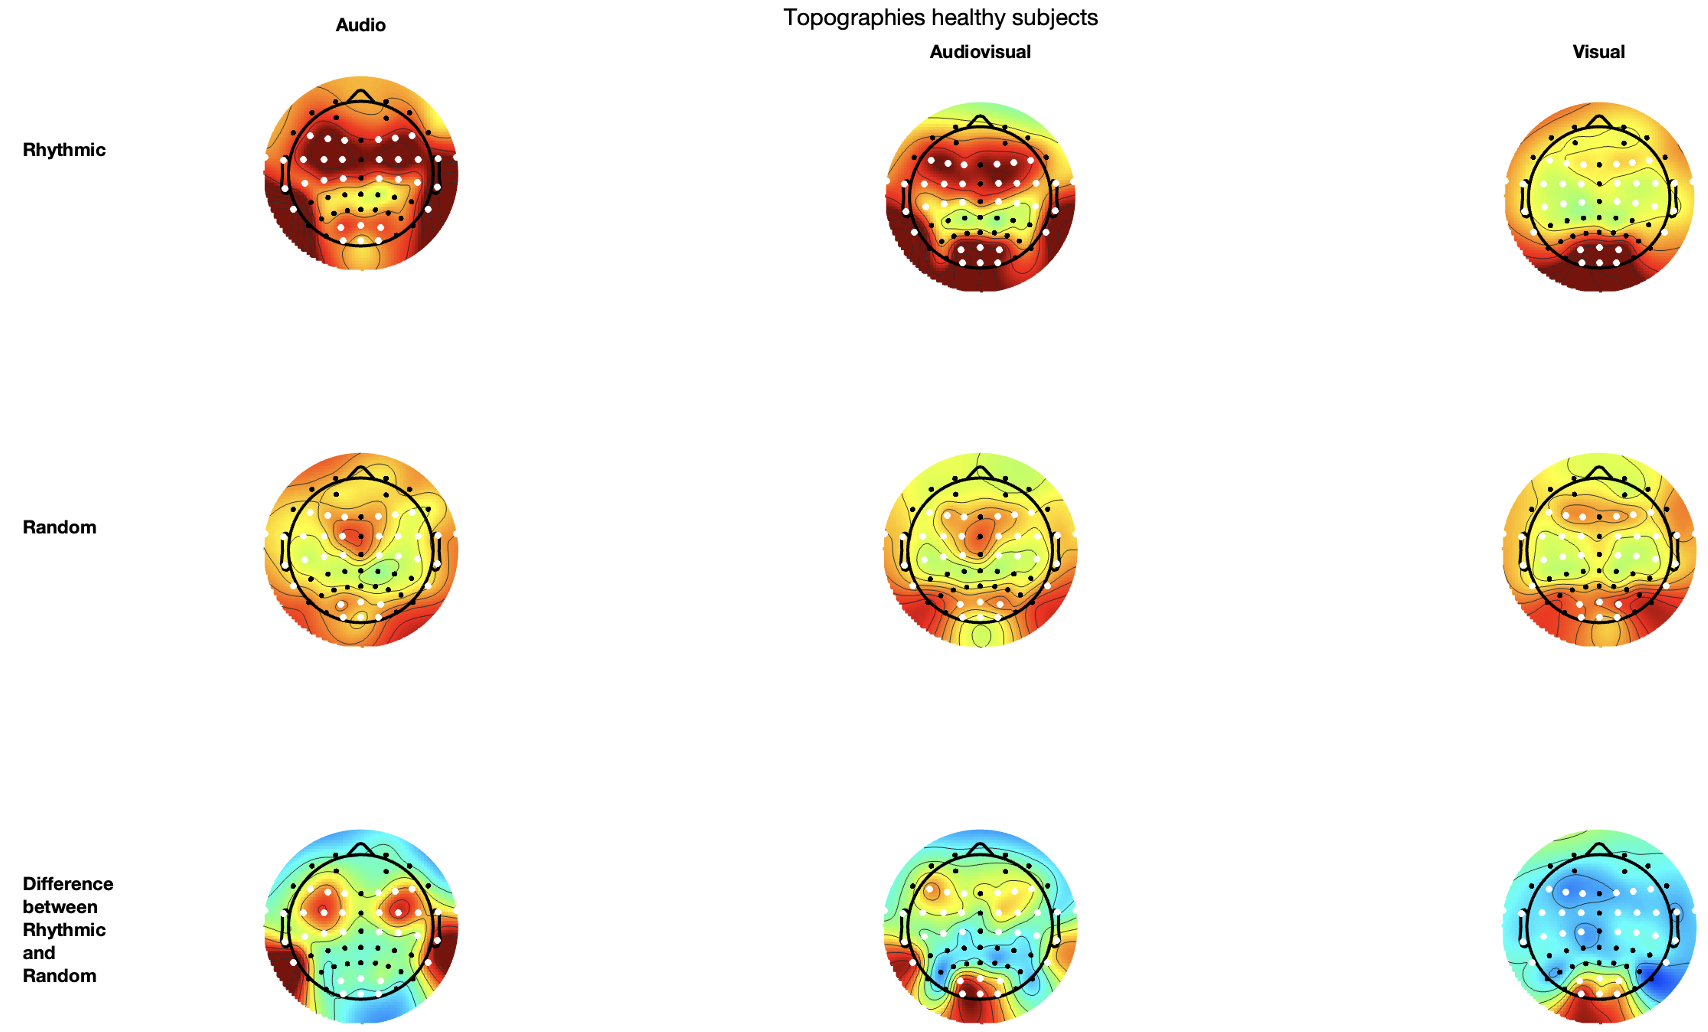
\includegraphics[width=0.95\textwidth]{healthy_images/topo.png}
    \caption{Topographies related to the activity in the control group}
    \label{fig: topographies control group}
\end{figure}
\begin{figure}[htbp]
    \centering
    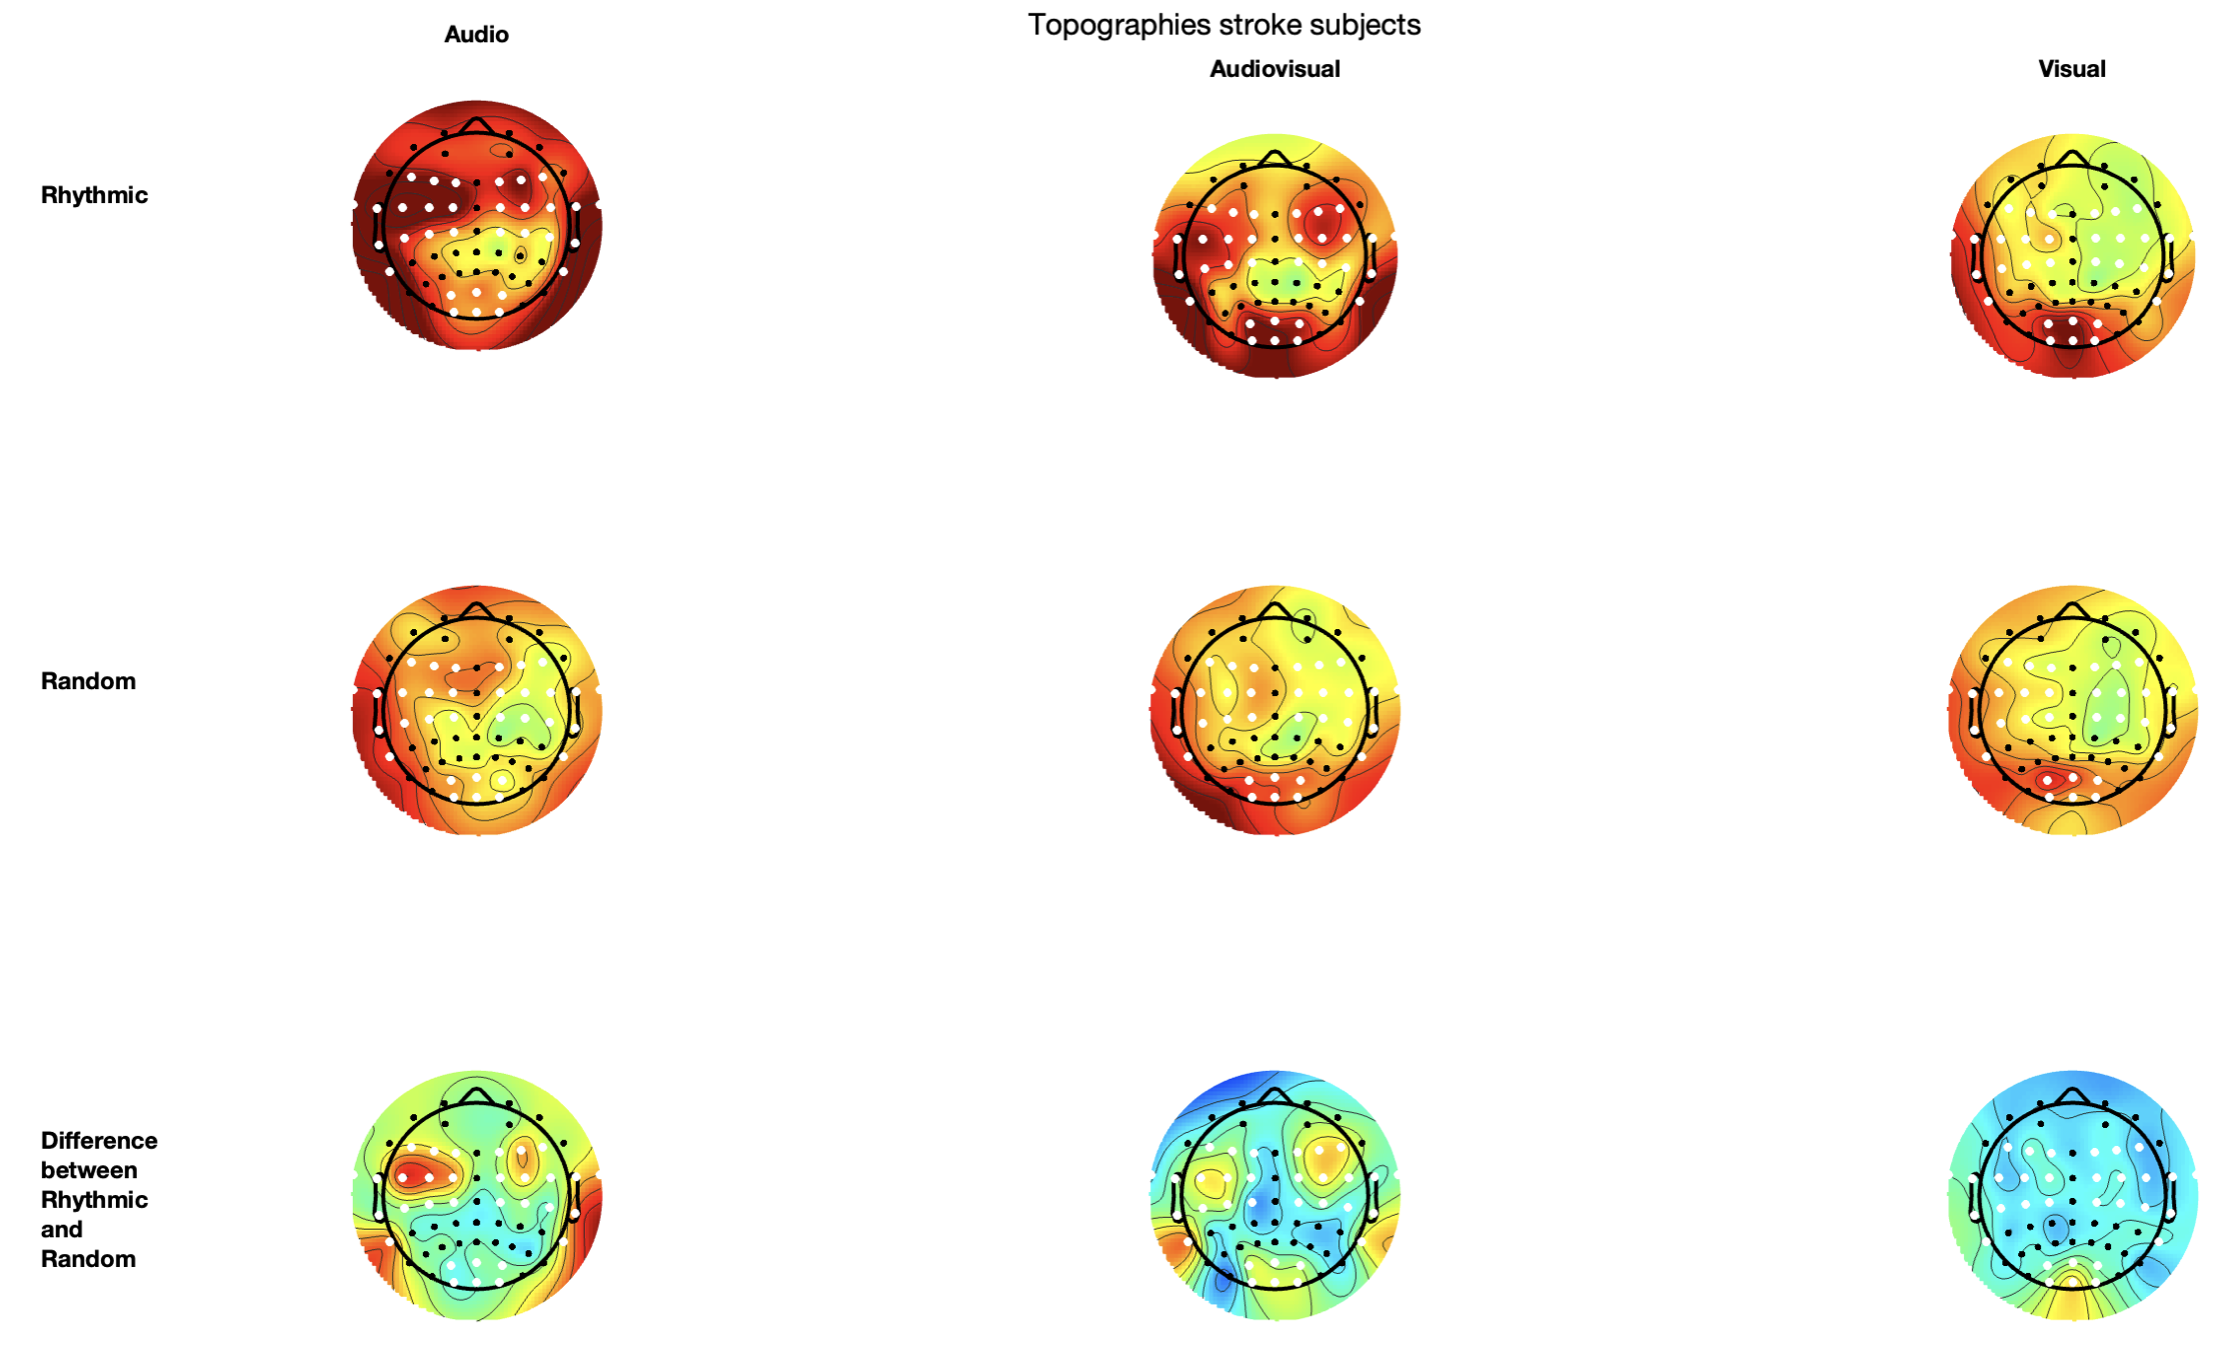
\includegraphics[width=0.85\textwidth]{stroke_images/topographies.png}
    \caption{Topographies related to the activity in stroke population}
    \label{fig: topographies stroke group}
\end{figure}
\begin{figure}[htbp]
    \centering
    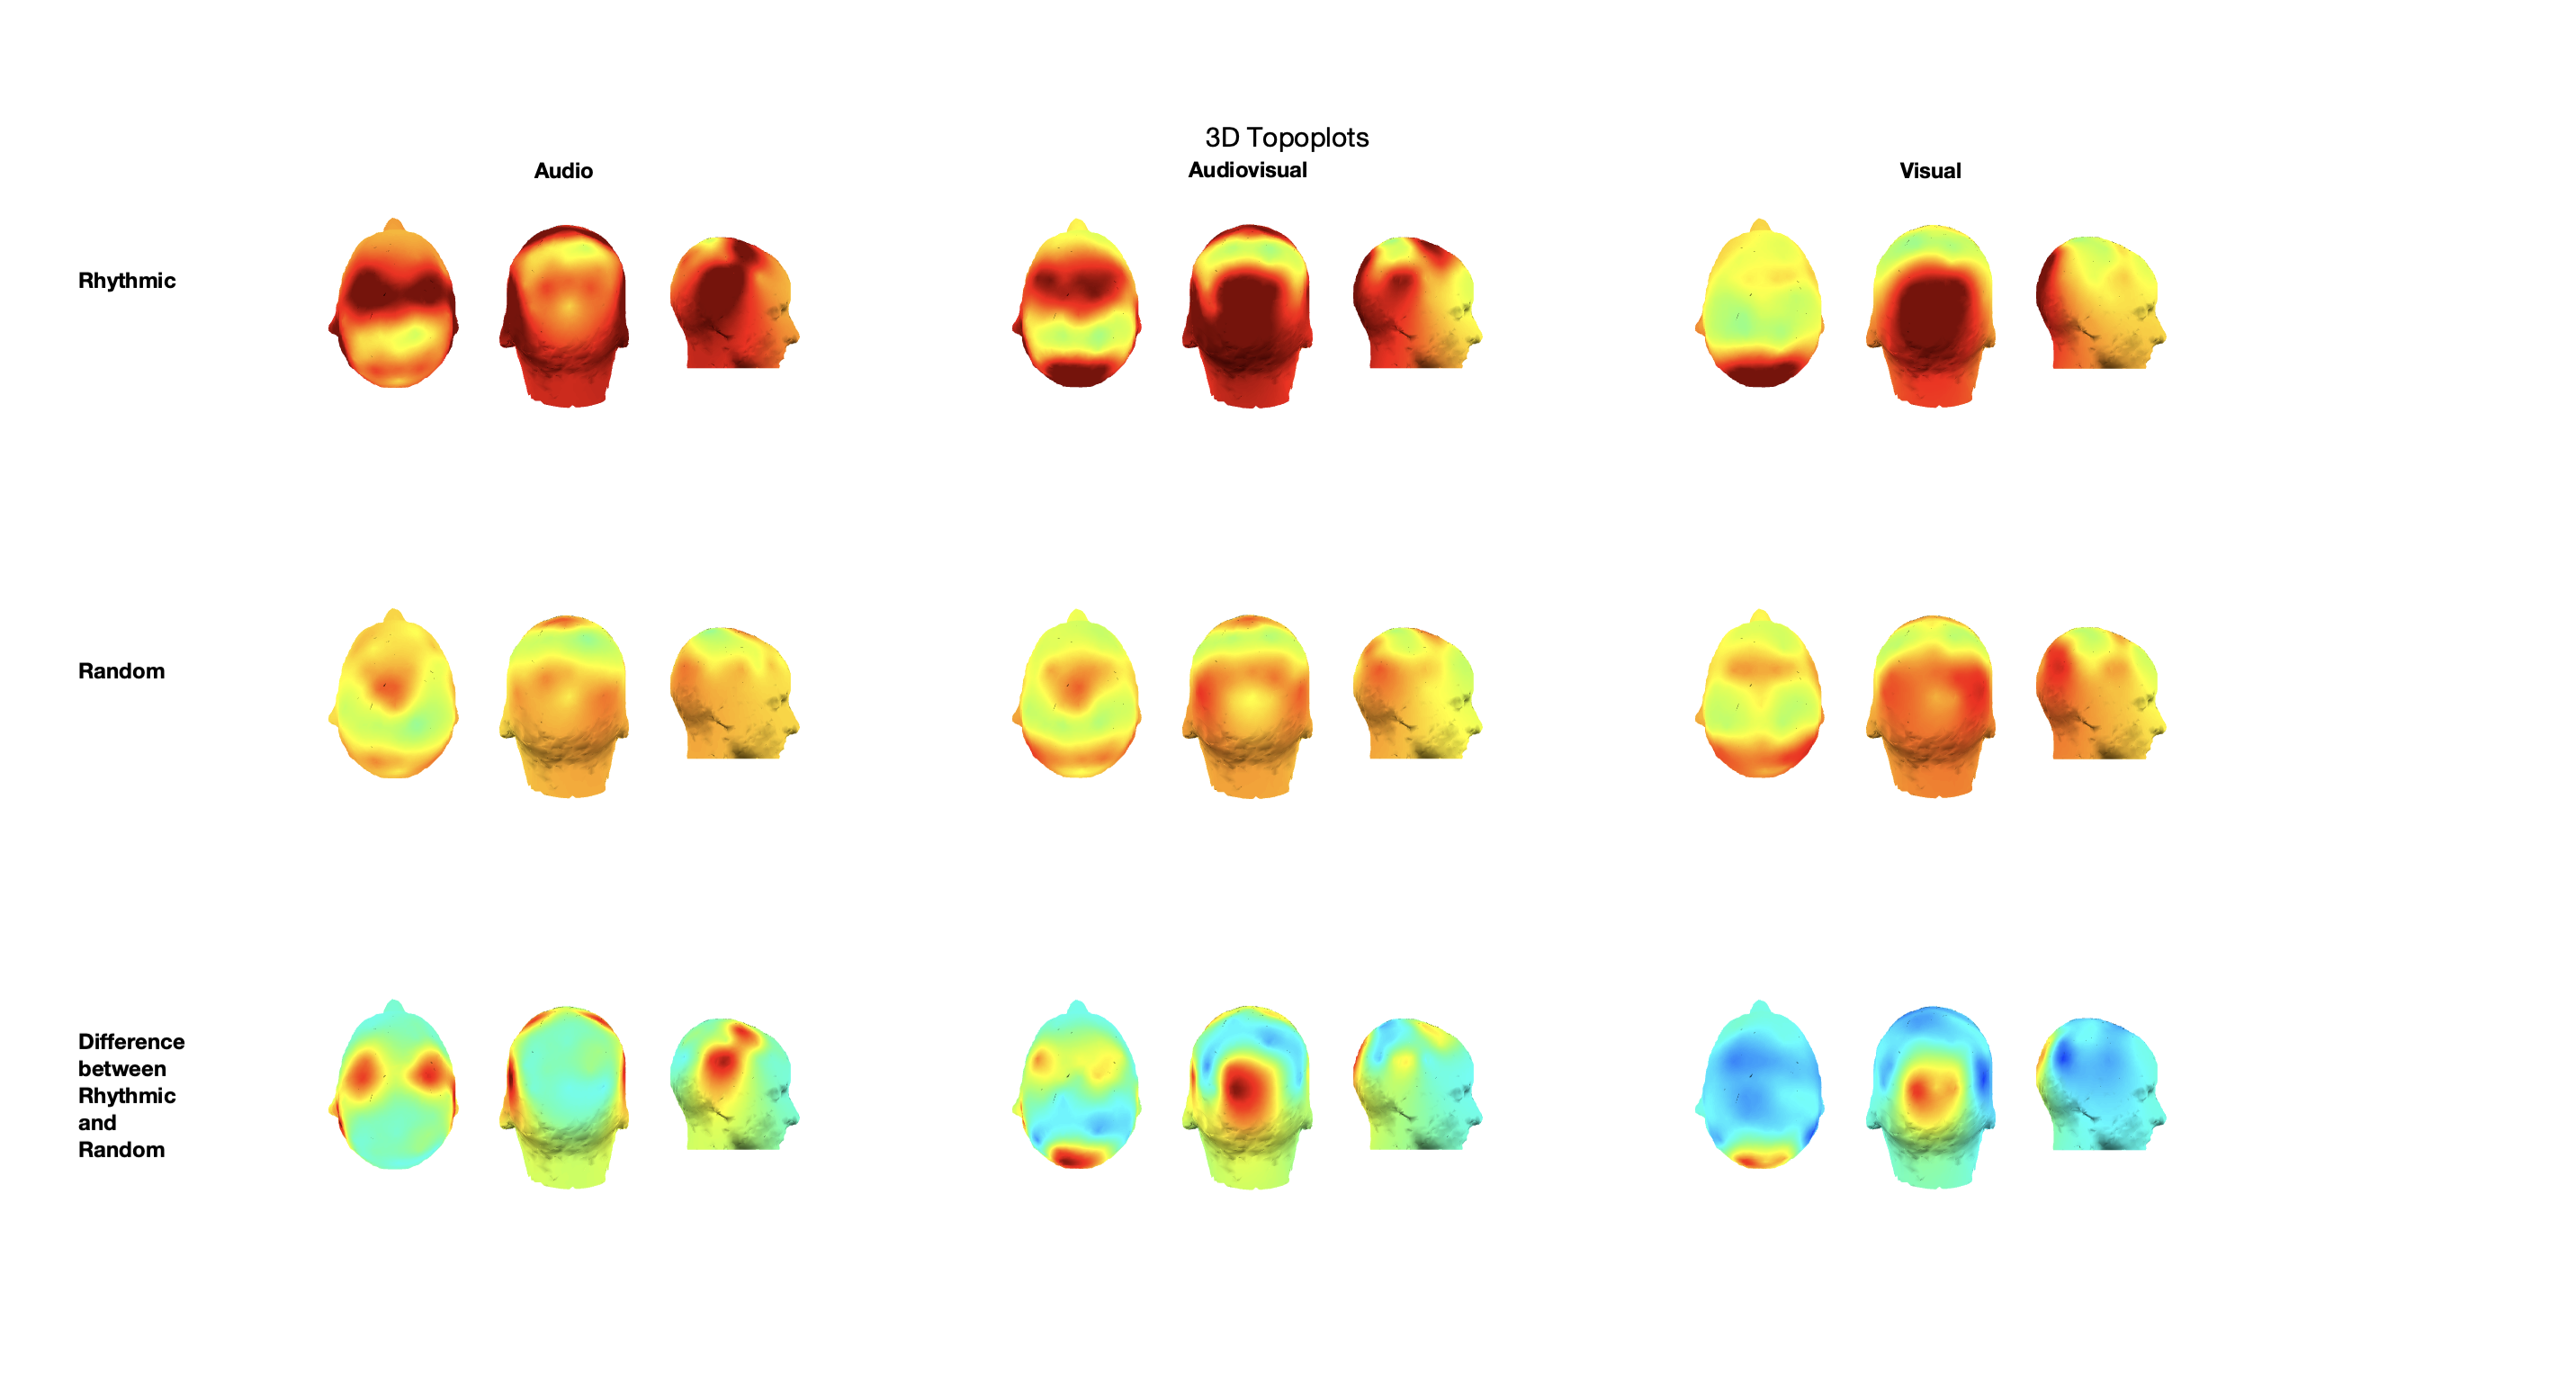
\includegraphics[width=0.85\textwidth]{healthy_images/3d_topo.png}
    \caption{3D topographies related to the activity in the control group}
    \label{fig: 3D topographies control group}   
\end{figure} 
\begin{figure}[htbp]
    \centering
    \includegraphics[width=0.85\textwidth]{stroke_images/3d_topographies.png}
    \caption{3D topographies related to the activity in stroke population}
    \label{fig: 3D topographies stroke group}   
\end{figure} 
\clearpage

\subsection*{Bar plots related to behavioral questions}
\subsubsection*{Control group}
\begin{figure}[H]
    \centering
    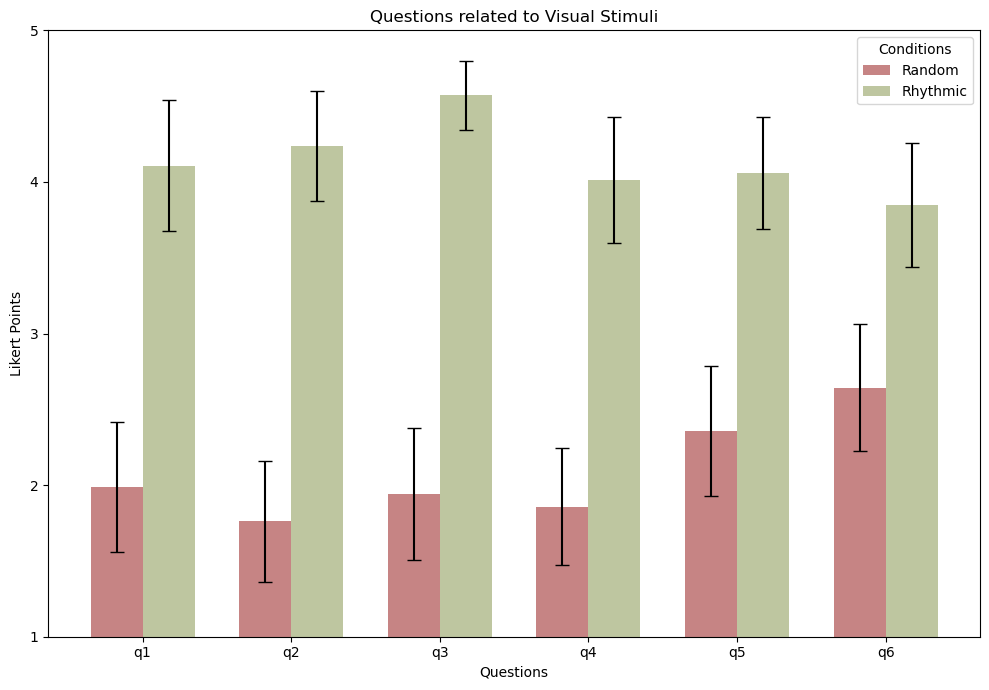
\includegraphics[width=0.85\textwidth]{bar_plots/plotbar_visual_h.png}
    \caption{Results of behavioral question in the visual condition in the control group}
    \label{fig: bar_visual_control} 
\end{figure} 
\begin{figure}[H]
    \centering
    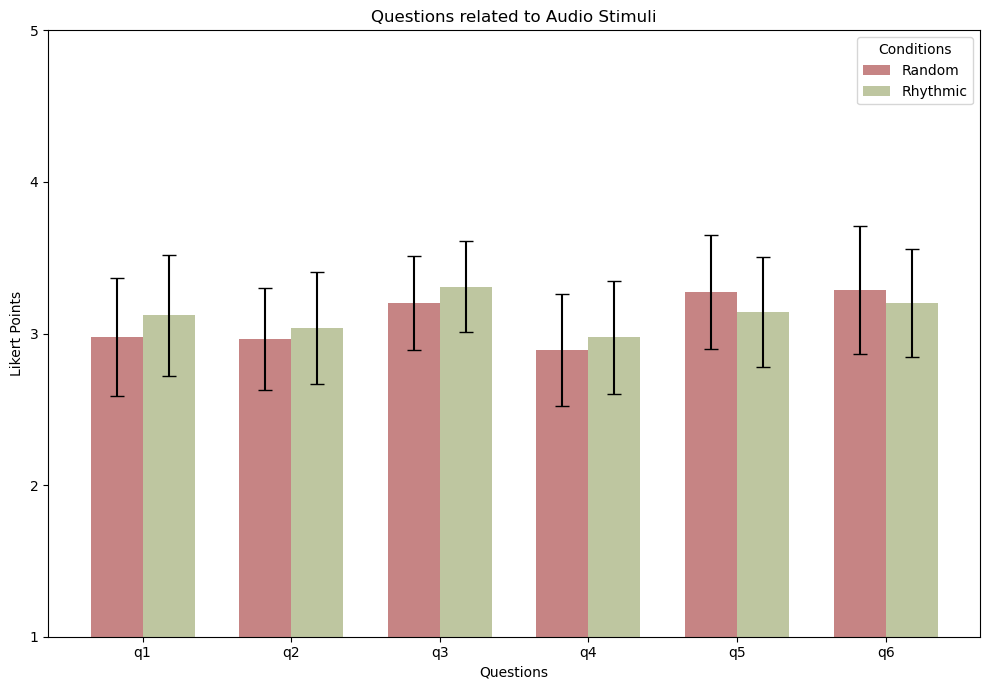
\includegraphics[width=0.85\textwidth]{bar_plots/plotbar_audio_h.png}
    \caption{Results of behavioral question in the audio condition in the control group}
    \label{fig: bar_audio_control} 
\end{figure} 
\begin{figure}[H]
    \centering
    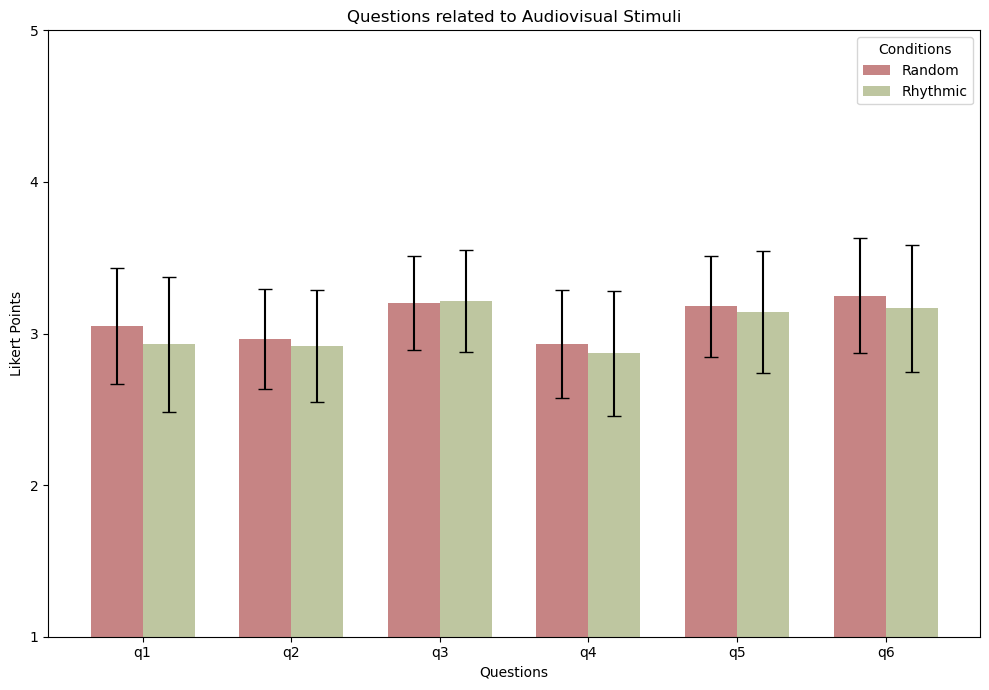
\includegraphics[width=0.85\textwidth]{bar_plots/plotbar_audiovisual_h.png}
    \caption{Results of behavioral question in the audiovisual condition in the control group}
    \label{fig: bar_audiovisual_control} 
\end{figure} 
\begin{figure}[H]
    \centering
    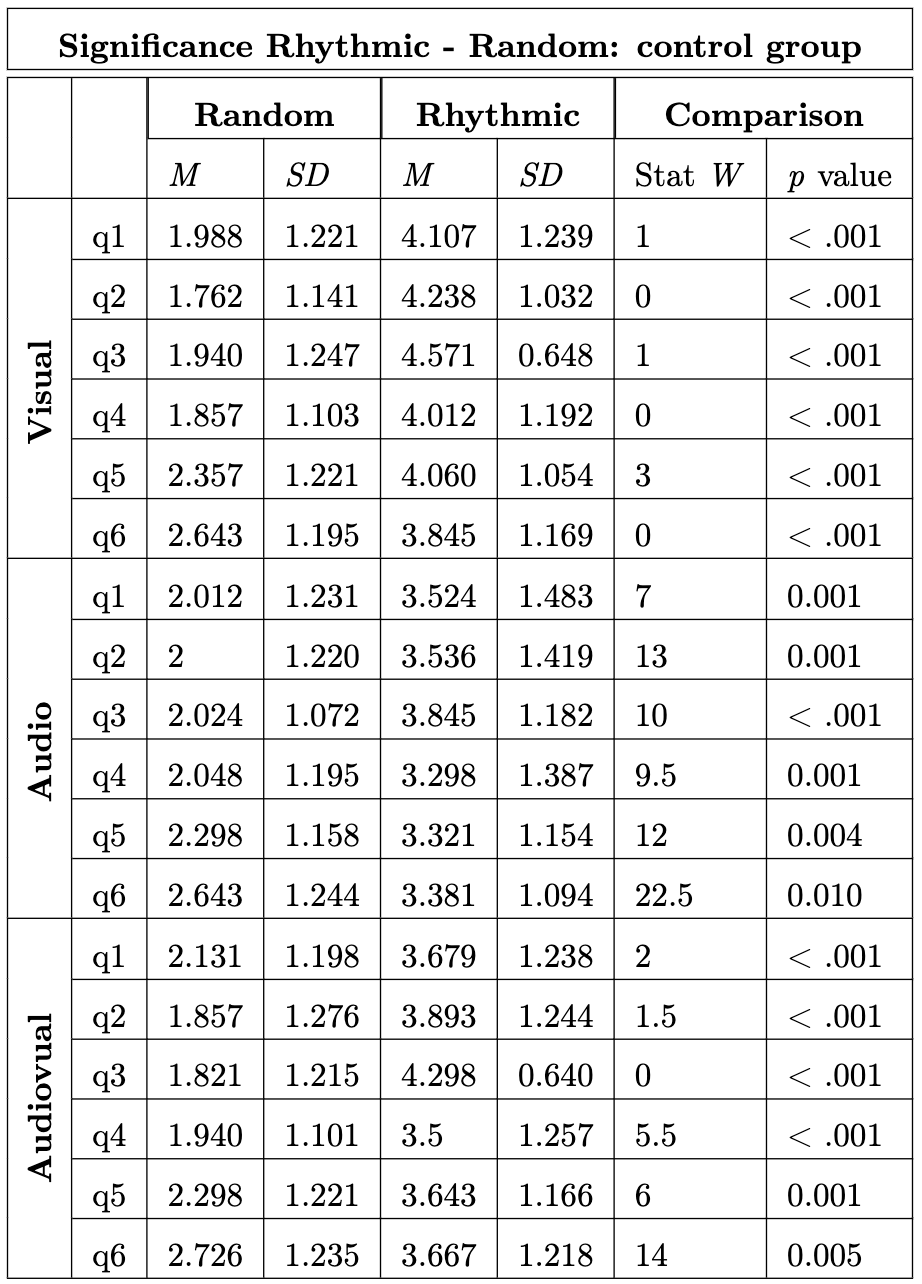
\includegraphics[width=0.45\textwidth]{significance_tables/control_group.png}
    \caption{Significance of the results of behavioral questions in the control group, using Wilcoxon Signed-Rank Test (\textit{W}); \textit{M} = mean; \textit{SD} = standard deviation}
    \label{fig: significance_control_pop} 
\end{figure} 

\clearpage
\subsubsection*{Stroke group}
\begin{figure}[H]
    \centering
    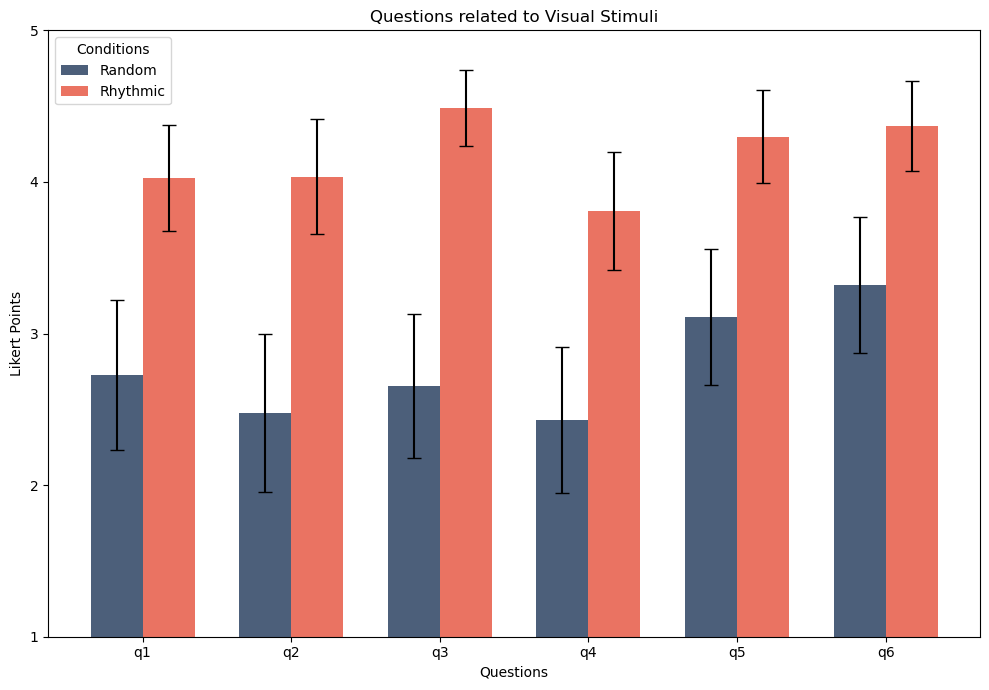
\includegraphics[width=0.85\textwidth]{bar_plots/plotbar_visual_s.png}
    \caption{Results of behavioral question in the visual condition in stroke population}
    \label{fig: bar_visual_stroke} 
\end{figure} 
\begin{figure}[H]
    \centering
    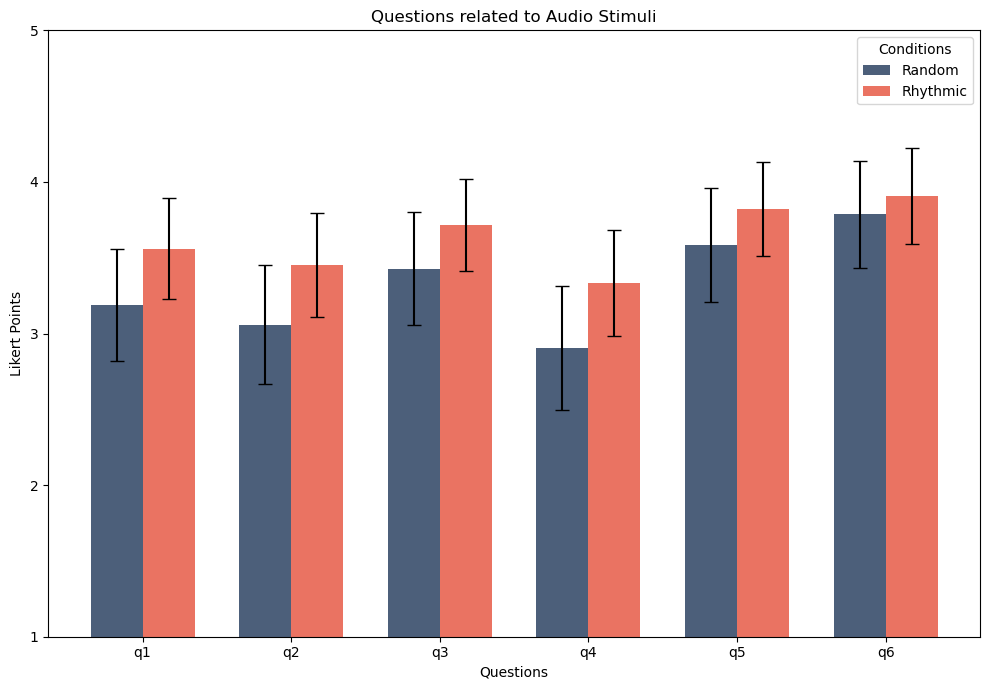
\includegraphics[width=0.85\textwidth]{bar_plots/plotbar_audio_s.png}
    \caption{Results of behavioral question in the audio condition in stroke population}
    \label{fig: bar_audio_stroke} 
\end{figure} 
\begin{figure}[H]
    \centering
    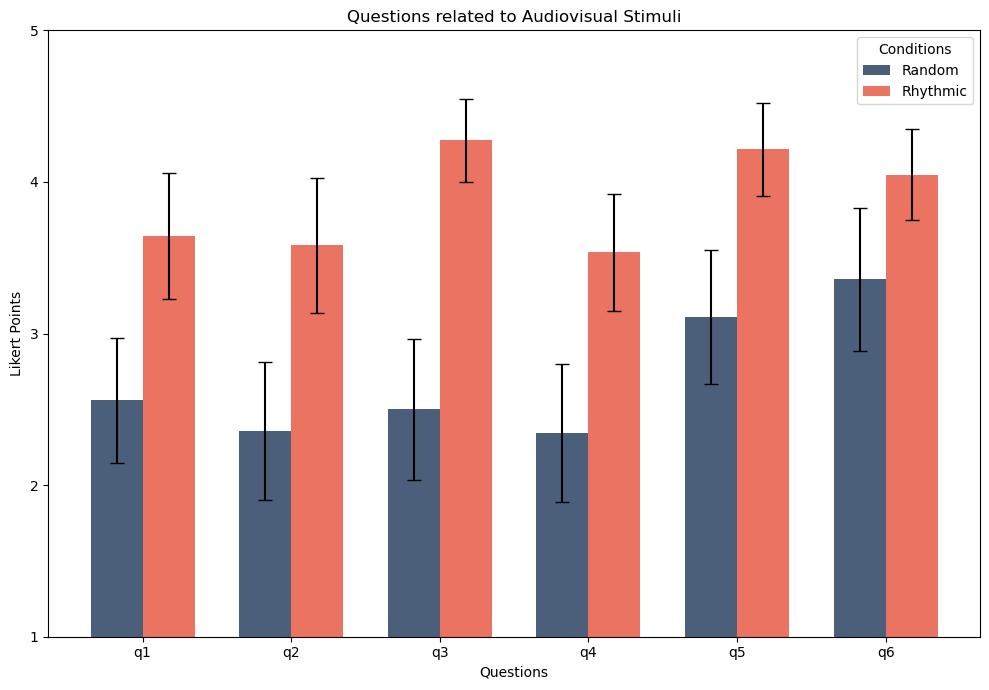
\includegraphics[width=0.85\textwidth]{bar_plots/plotbar_audiovisual_s.png}
    \caption{Results of behavioral question in the audiovisual condition in stroke population}
    \label{fig: bar_audiovisual_stroke} 
\end{figure} 
\begin{figure}[H]
    \centering
    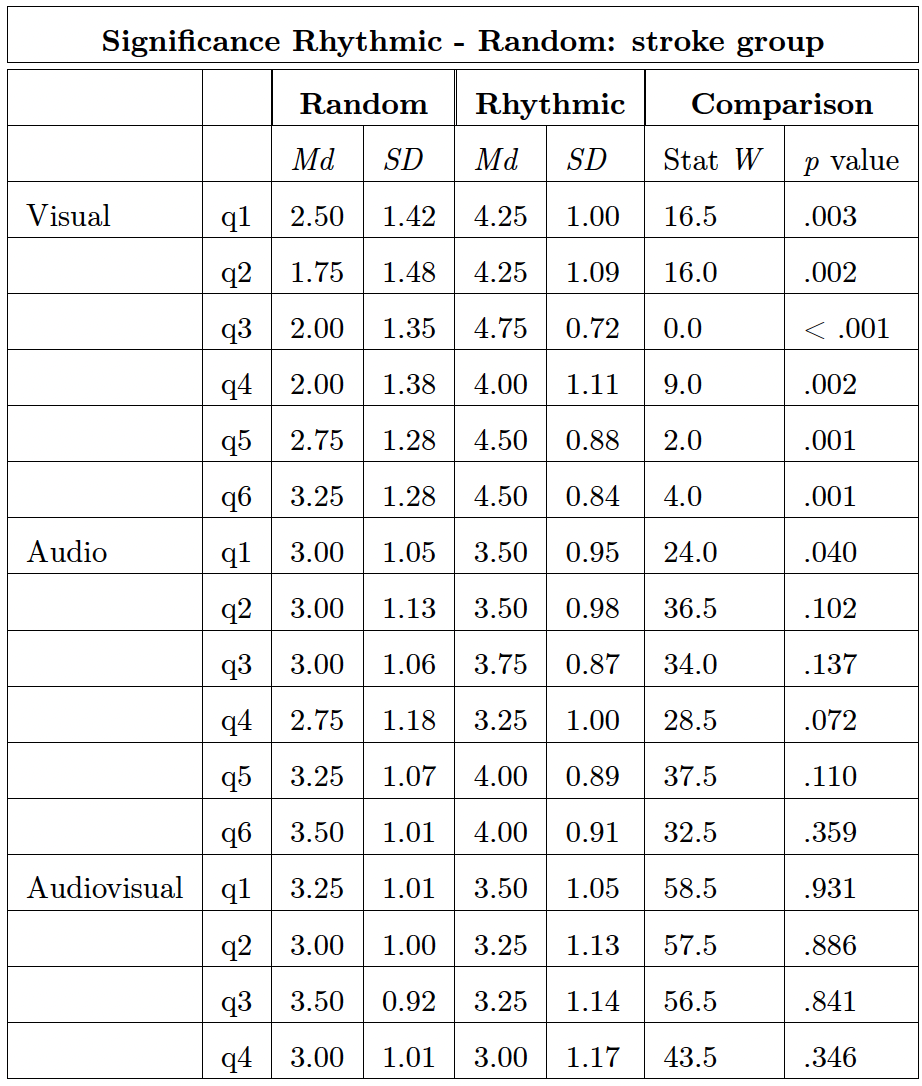
\includegraphics[width=0.45\textwidth]{significance_tables/stroke_group.png}
    \caption{Significance of the results of behavioral questions in the stroke group, using Wilcoxon Signed-Rank Test (\textit{W}); \textit{M} = mean; \textit{SD} = standard deviation}
    \label{fig: significance_stroke_pop} 
\end{figure} 

\clearpage
\subsubsection*{Total results mean}
\begin{figure}[H]
    \centering
    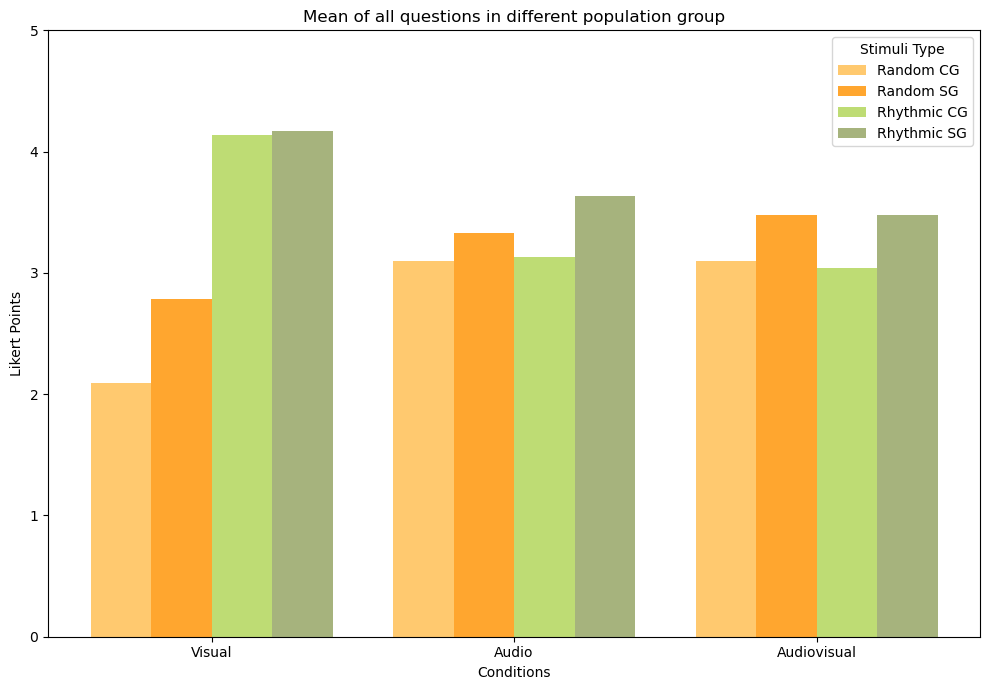
\includegraphics[width=0.85\textwidth]{bar_plots/mean stroke and control.png}
    \caption{Mean of the results of all behavioral question divided by population groups (CG = control group; SG = stroke group)}
    \label{fig: mean_population_condition} 
\end{figure} 
\begin{figure}[H]
    \centering
    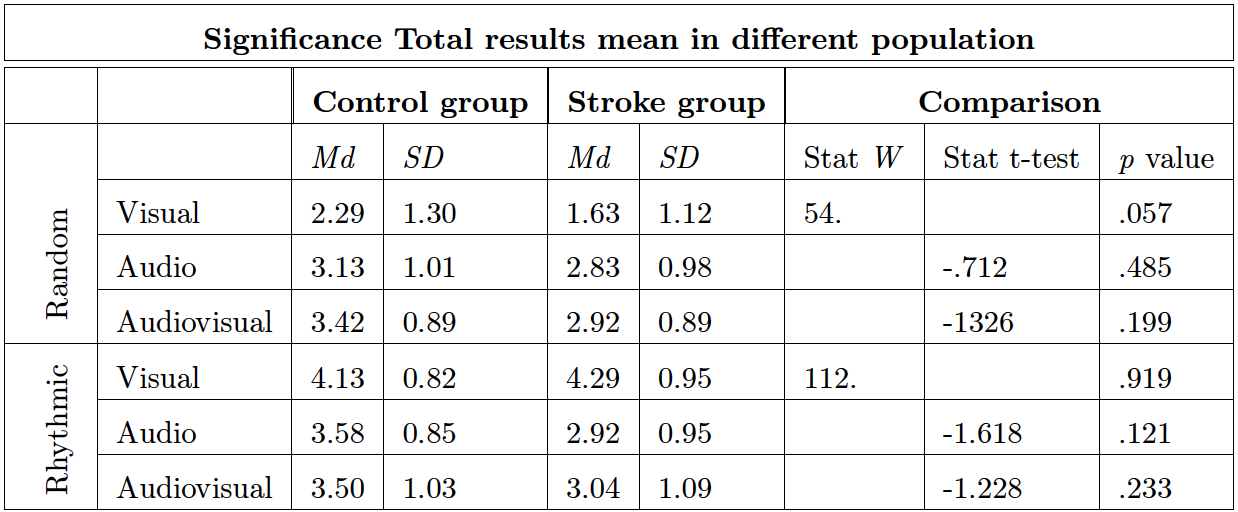
\includegraphics[width=0.70\textwidth]{significance_tables/tot_mean_pop.png}
    \caption{Significance of the results of all behavioral questions, comparing different population groups, using Wilcoxon Signed-Rank Test (\textit{W}) or Paired Samples t-Test (\textit{t}); \textit{M} = mean; \textit{SD} = standard deviation}
    \label{fig: significance_total_mean_pop} 
\end{figure} 

\clearpage
\subsection*{Correlation between brain activation and behavioral questions}
\subsubsection*{Control group}
\begin{figure}[H]
    \centering
    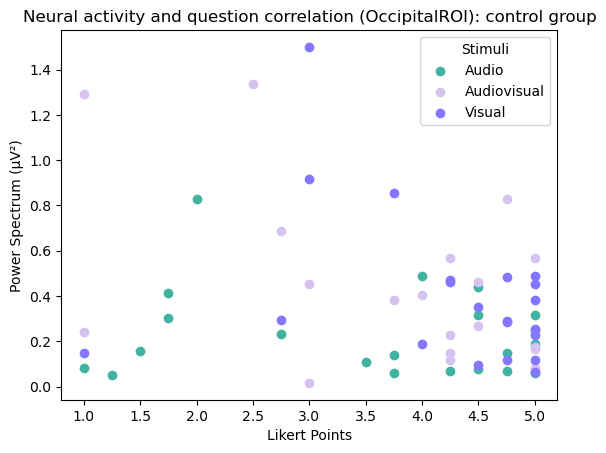
\includegraphics[width=0.75\textwidth]{scatter_plots/h_occipital_q2.png}
    \caption{Correlation between neural activation and behavioral question in the control group}
    \label{fig: correlation q2 occipitalROI: control group} 
\end{figure}
\begin{figure}[H]
    \centering
    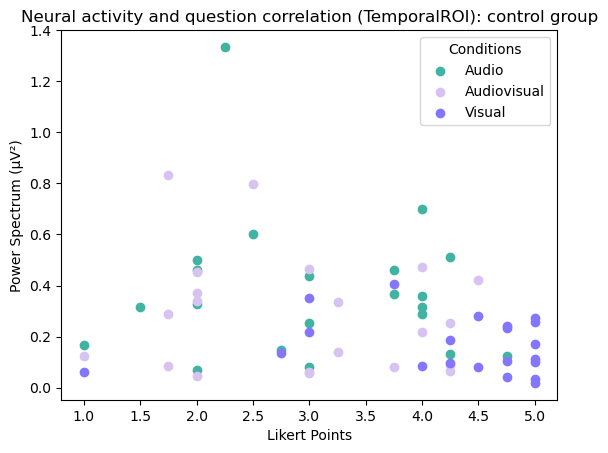
\includegraphics[width=0.75\textwidth]{scatter_plots/h_temporal_q2.png}
    \caption{Correlation between neural activation and behavioral questions in the stroke population}
    \label{fig: correlation q2 temporalROI: control group} 
\end{figure}
\begin{figure}[H]
    \centering
    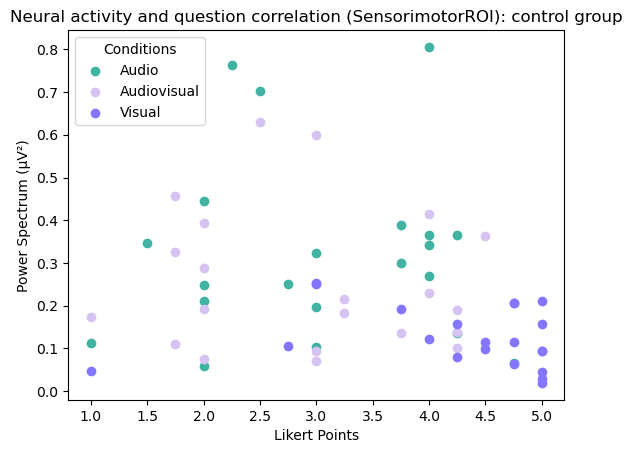
\includegraphics[width=0.75\textwidth]{scatter_plots/h_sensorimotor_q2.png}
    \caption{Correlation between neural activation and behavioral questions in the stroke population}
    \label{fig: correlation q2 sensorimotorROI: control group} 
\end{figure}
\begin{figure}[H]
    \centering
    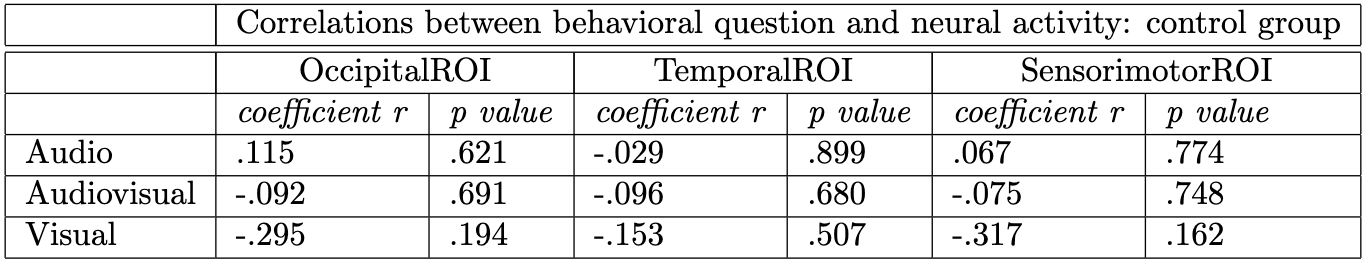
\includegraphics[width=0.75\textwidth]{scatter_plots/correlation_q2_control.png}
    \caption{Correlation values: Spearman correlation coefficient \textit{r} and \textit{p} value}
    \label{fig: correlation values q2: control} 
\end{figure}

\clearpage
\subsubsection*{Stroke group}
\begin{figure}[H]
    \centering
    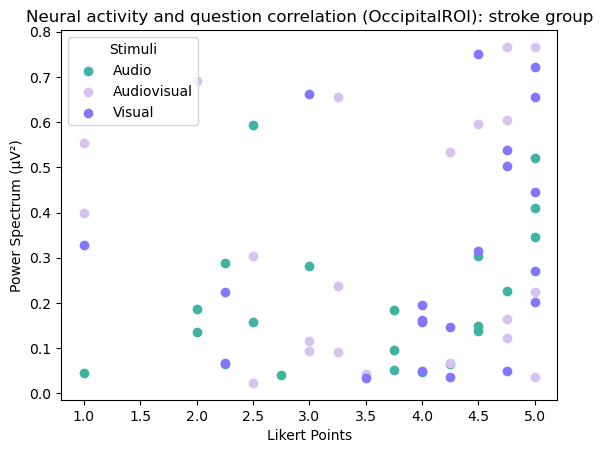
\includegraphics[width=0.75\textwidth]{scatter_plots/s_occipital_q2.png}
    \caption{Correlation between neural activation and behavioral question in the control group}
    \label{fig: correlation q2 occipitalROI: stroke group} 
\end{figure}
\begin{figure}[H]
    \centering
    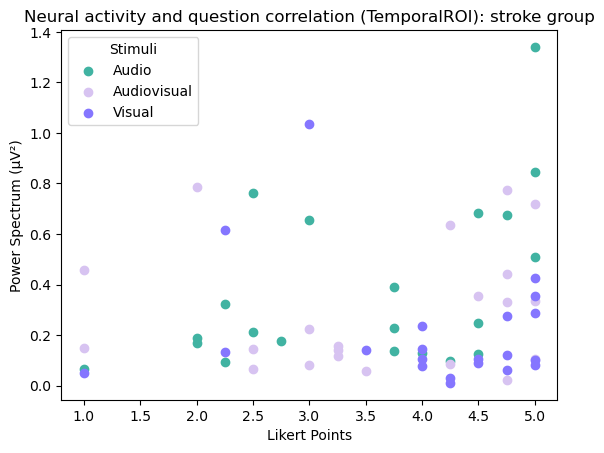
\includegraphics[width=0.75\textwidth]{scatter_plots/s_temporal_q2.png}
    \caption{Correlation between neural activation and behavioral questions in the stroke population}
    \label{fig: correlation q2 temporalROI: stroke group} 
\end{figure}
\begin{figure}[H]
    \centering
    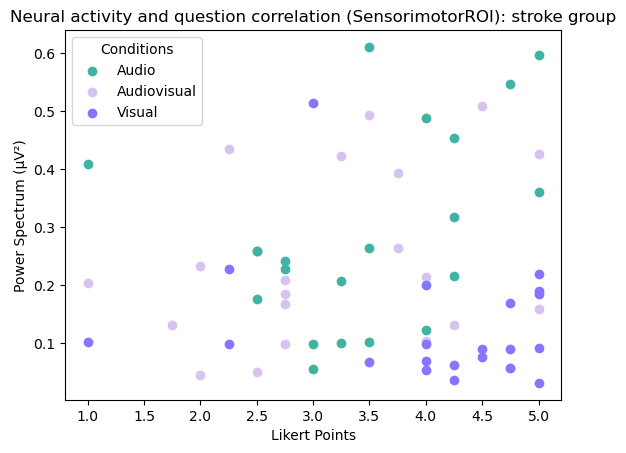
\includegraphics[width=0.75\textwidth]{scatter_plots/s_sensorimotor_q2.png}
    \caption{Correlation between neural activation and behavioral questions in the stroke population}
    \label{fig: correlation q2 sensorimotorROI: stroke group} 
\end{figure}
\begin{figure}[H]
    \centering
    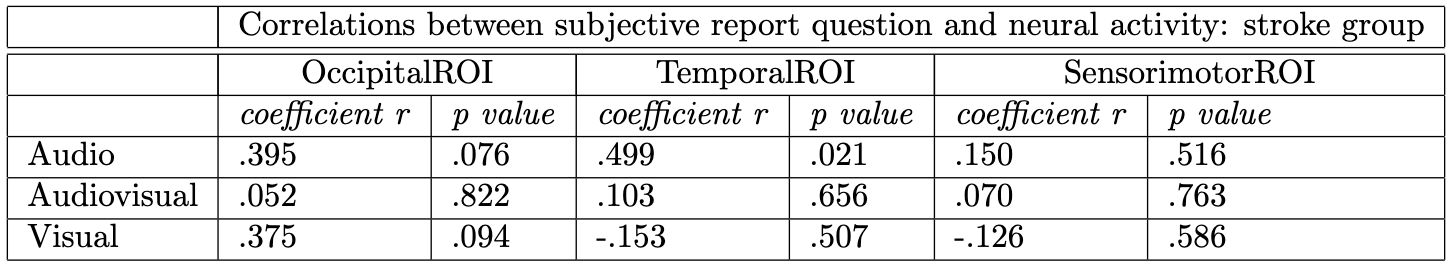
\includegraphics[width=0.75\textwidth]{scatter_plots/correlation_q2_stroke.png}
    \caption{Correlation values: Pearson correlation coefficient \textit{r} and \textit{p} value}
    \label{fig: correlation values q2: stroke} 
\end{figure}

\clearpage
\subsection*{Correlation between physical activity and brain activation}
\begin{figure}[H]
    \centering
    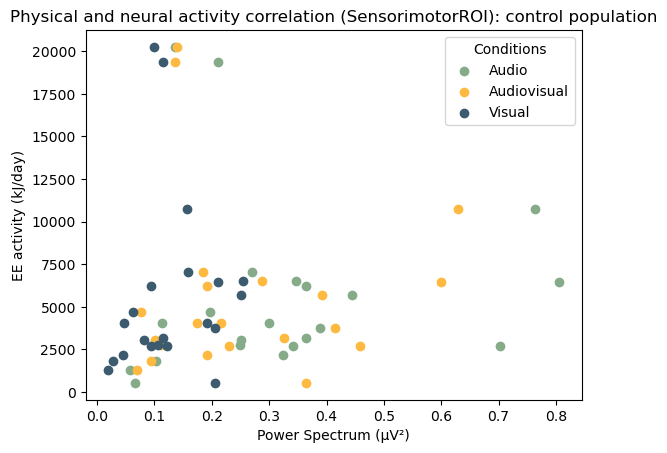
\includegraphics[width=0.75\textwidth]{scatter_plots/h_sensorimotor_activeq.png}
    \caption{Correlation between activity and neural activation in the control group}
    \label{fig: correlation activeq control} 
\end{figure}
\begin{figure}[H]
    \centering
    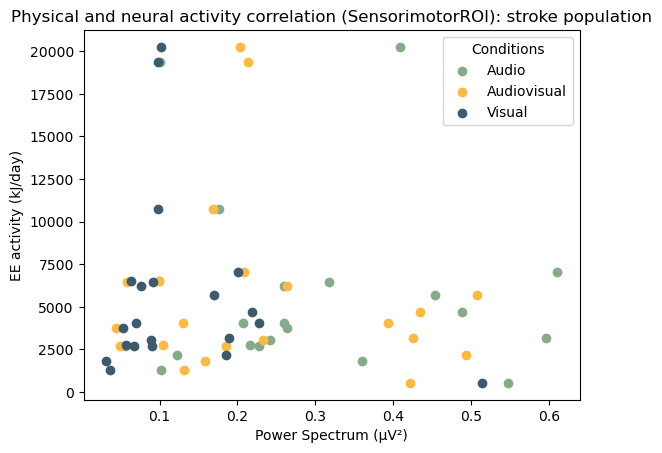
\includegraphics[width=0.75\textwidth]{scatter_plots/s_sensorimotor_activeq.png}
    \caption{Correlation between activity and neural activation in the stroke population}
    \label{fig: correlation activeq stroke} 
\end{figure}
\begin{figure}[H]
    \centering
    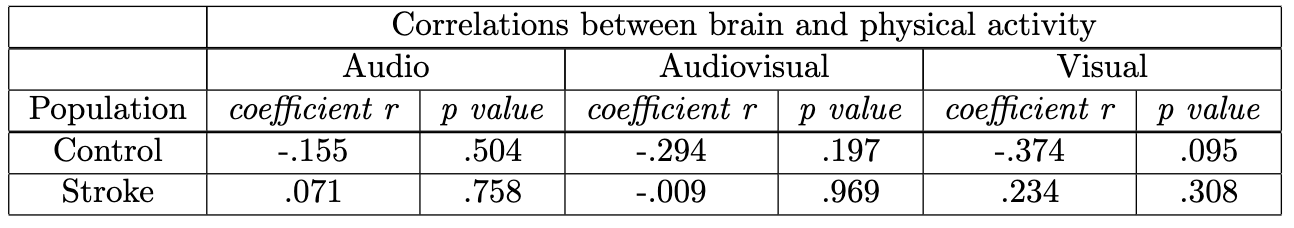
\includegraphics[width=0.75\textwidth]{significance_tables/correlation_activeq_.png}
    \caption{Correlation values: Spearman's correlation coefficient \textit{r} and \textit{p} value}
    \label{fig: significance correlation activeq} 
\end{figure}